\section{Work plan}

To spend our time as efficient as possible we decided to make a plan of how much progress was to be done on the fuel cell the following weeks. The work plan gave us deadlines for what was to be done and gave us an easy way to keep track of that was to be done each week.

\begin{center}
    \begin{table}[h]
        \centering
        \begin{tabular}{|c|c|}
        \hline
        Week & Time \\
        \hline
        1 & Concept brainstorming and sketching  \\ 
        \hline
        2 & Creating modulation in Solidworks \\
        \hline
        3 & 3D printing housing part \\
        \hline
        4 & Assembling and testing \\ 
        \hline
     \end{tabular}
     \caption{Plan of progress}
     \label{tab:Workplan}
    \end{table}
\end{center}



\section{Modulation of housing parts}

We used the program Solidworks to modulate the fuel cell housing parts. The housing parts dimensions were determined on the bases of the fuel cell chamber as we needed enough space between the chamber and the outer dimensions of the housing parts for the sealant to have enough space to seal properly. The maximum parameter we were given for the fuel cell itself was 50x50mm therefor the chamber dimensions were set for us. We decided that 25mm spacing between the chamber and the outer dimensions of the fuel cell would be enough space to seal the two parts together. Thereby making the fuel cells outer dimensions 100x100mm. To not use excessive amounts of filament and time while 3D printing, and still make the two housing parts strong enough to withstand wear and tear, we decided that a thickness of 10mm of would be sufficient. As the fuel cell chamber needed a volume that would hold two metal plates with a thickness
 of.. and the fuel cell itself, the depth in each part was sett to be 2mm. Making the total dimensions of the fuel cell housing to be 100x100x20mm with a chamber of 50x50x4mm.


To pin the two housing parts together we decided to use M6 bolts. There were made two holes on each side of the housing parts, making a total of eight bolt holes per part. To easily fit the M6 bolts we made the bolthole diameter 6,5mm as the M6 bolts have a diameter of 6mm. The middle bolthole was modeled and 3D printed with a diameter of 10mm but was threaded to fit an M12 bolt after the parts were printed. 

\section{The 3D printer}

\subsection{Ultimaker 2 Go/2+}

The printers used in this project are the Ultimaker 2 Go and Ultimaker 2+. The Ultimaker 2 Go is a small printer, able to print builds up to 120 x 120 x 115 mm. For this project this printer was used to print prototypes and to learn how to use the 3D printers. The reason for this is the high printig speed and high availability at the lab. Due to safety margins on the printer it was not possible for us to print the full scale housing on this printer. The fact sheet for the printer can be found in appendix C.

The Ulitmake 2+ has the ability to print builds up to 223 x 223 x 205 mm. This was the printer used to print the final housing parts for the PEM fuel cell. 

\subsection{Filament}

The filament we used is Polylactic acid (PLA) plastic. The filament used has a printing temperature of 180-210 \textdegree C and a melting point at 145-160 \textdegree C. The technical sheet for the fillament can be found in appendix D.

\subsection{Ultimaker Cura}

To print the 3D model created in Solidworks the slicer program Ultimaker Cura was used. The slicer program turns the 3D model into several "slices" which the printer then can print. Ultimaker Cura also generated the necessary amount of support structure to pint the housing parts. 

\section{Printing the model}

\subsection{Printing of draft housing} 

After completing the modeling in Solidworks, we decided to print scaled down version of one side of the housing. We scaled the oxygen side of the housing down to 40\% of the original size and printed it. Our goal by printing a small scale model was to look for design errors we could not find on the computer model. Printing the draft was also a good way to learn how the 3D printers worked as none of us had used them before.

The first draft print did not go as planed. After about half an hour the printer failed and we had to abort the printing process. The results of the first draft print can be seen on the picture below, figure \ref{fig:Draft1}.


\begin{figure}[ht]
    \centering
    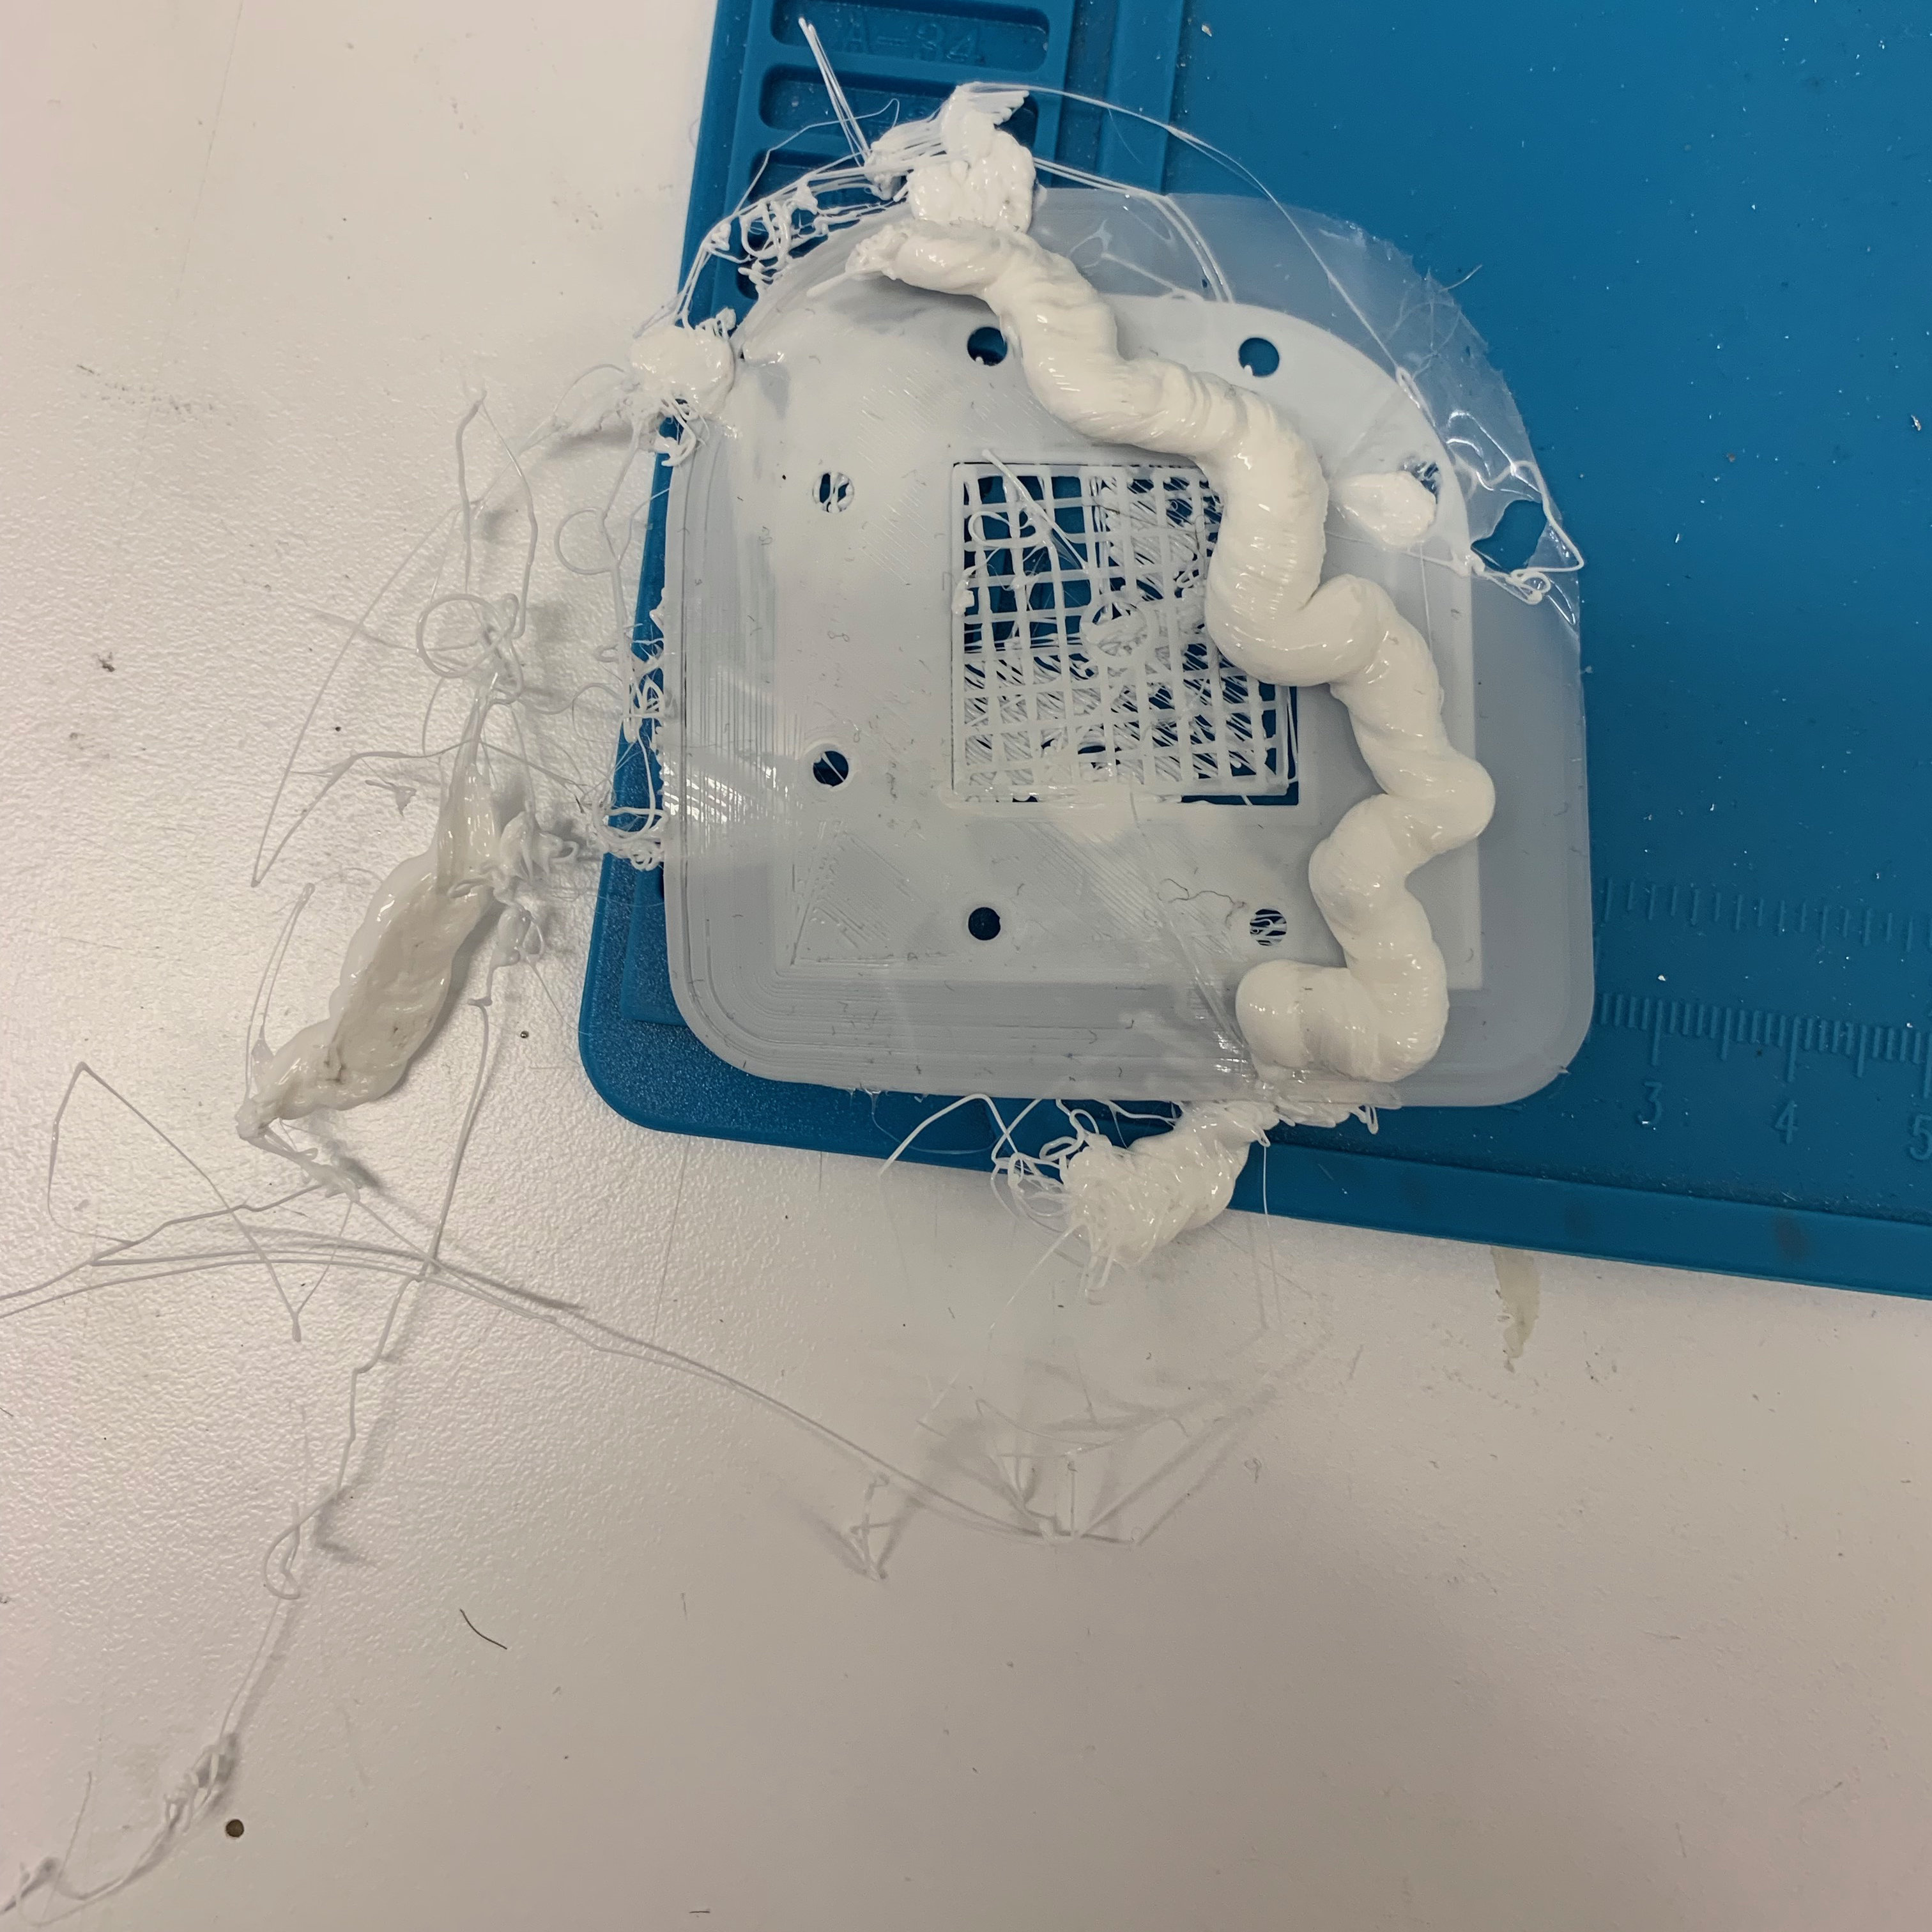
\includegraphics[width=0.40\textwidth]{DIV./Bilder/Draft1.jpg}
    \caption{Picture of the first draft print}
    \label{fig:Draft1}
\end{figure}

As the first draft print failed, we started to look for errors in the printing file and errors on the 3D printer. What we found was that the model had moved on the building plate during the printing. To fix this problem we covered the top of the building plate in masking tape to create more friction. We also made a new printing file just to be on the safe side. 

After an hour of printing the small scale model was complete. This time the result was good. We got a great look at how our design was going to look like. We did not find anything that we needed to change before printing the full scale model.

\subsection{Printing the housing}

\subsubsection{Scaled Prototype}

As the 40\% scale housing looked fine we proceeded by creating the printing file for the full size housing. In order to use the least amount of time possible on waiting for 3D printers to become available we decided to print both the hydrogen and oxygen side at the same time. 

\subsubsection{First print}

After 24 hours of printing we discovered that the print had failed. The tape had separated from the building plate. As a result of this the sides of the housing had begun to curve and deform. There was no reason til continue the print, and we aborted the print. The building plate was cleaned and the print was scraped. 

\begin{figure}[ht]
    \centering
    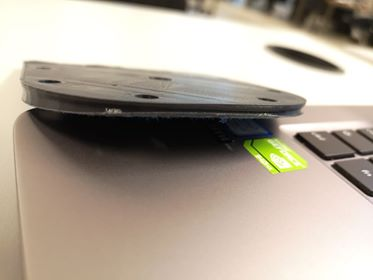
\includegraphics[width=0.6\textwidth]{DIV./Bilder/Firstprint.jpg}
    \caption{Picture of the first print}
    \label{fig:Print1}
\end{figure}

\subsubsection{Final print}

After the print failed we looked for errors. Our conclusions was that due to the large surface area of the building plate being printed on the amount of heat had affected the tape. We decided to print each side of the fuel cell by themselves and build some support structure under the housing part. By building the support structure we hoped it let some of the heat dissipate. Figure \ref{fig:Housingprint} is taken during the printing of the oxygen side of the housing and shows the support structure printed under the housing part.

\begin{figure}[ht]
    \centering
    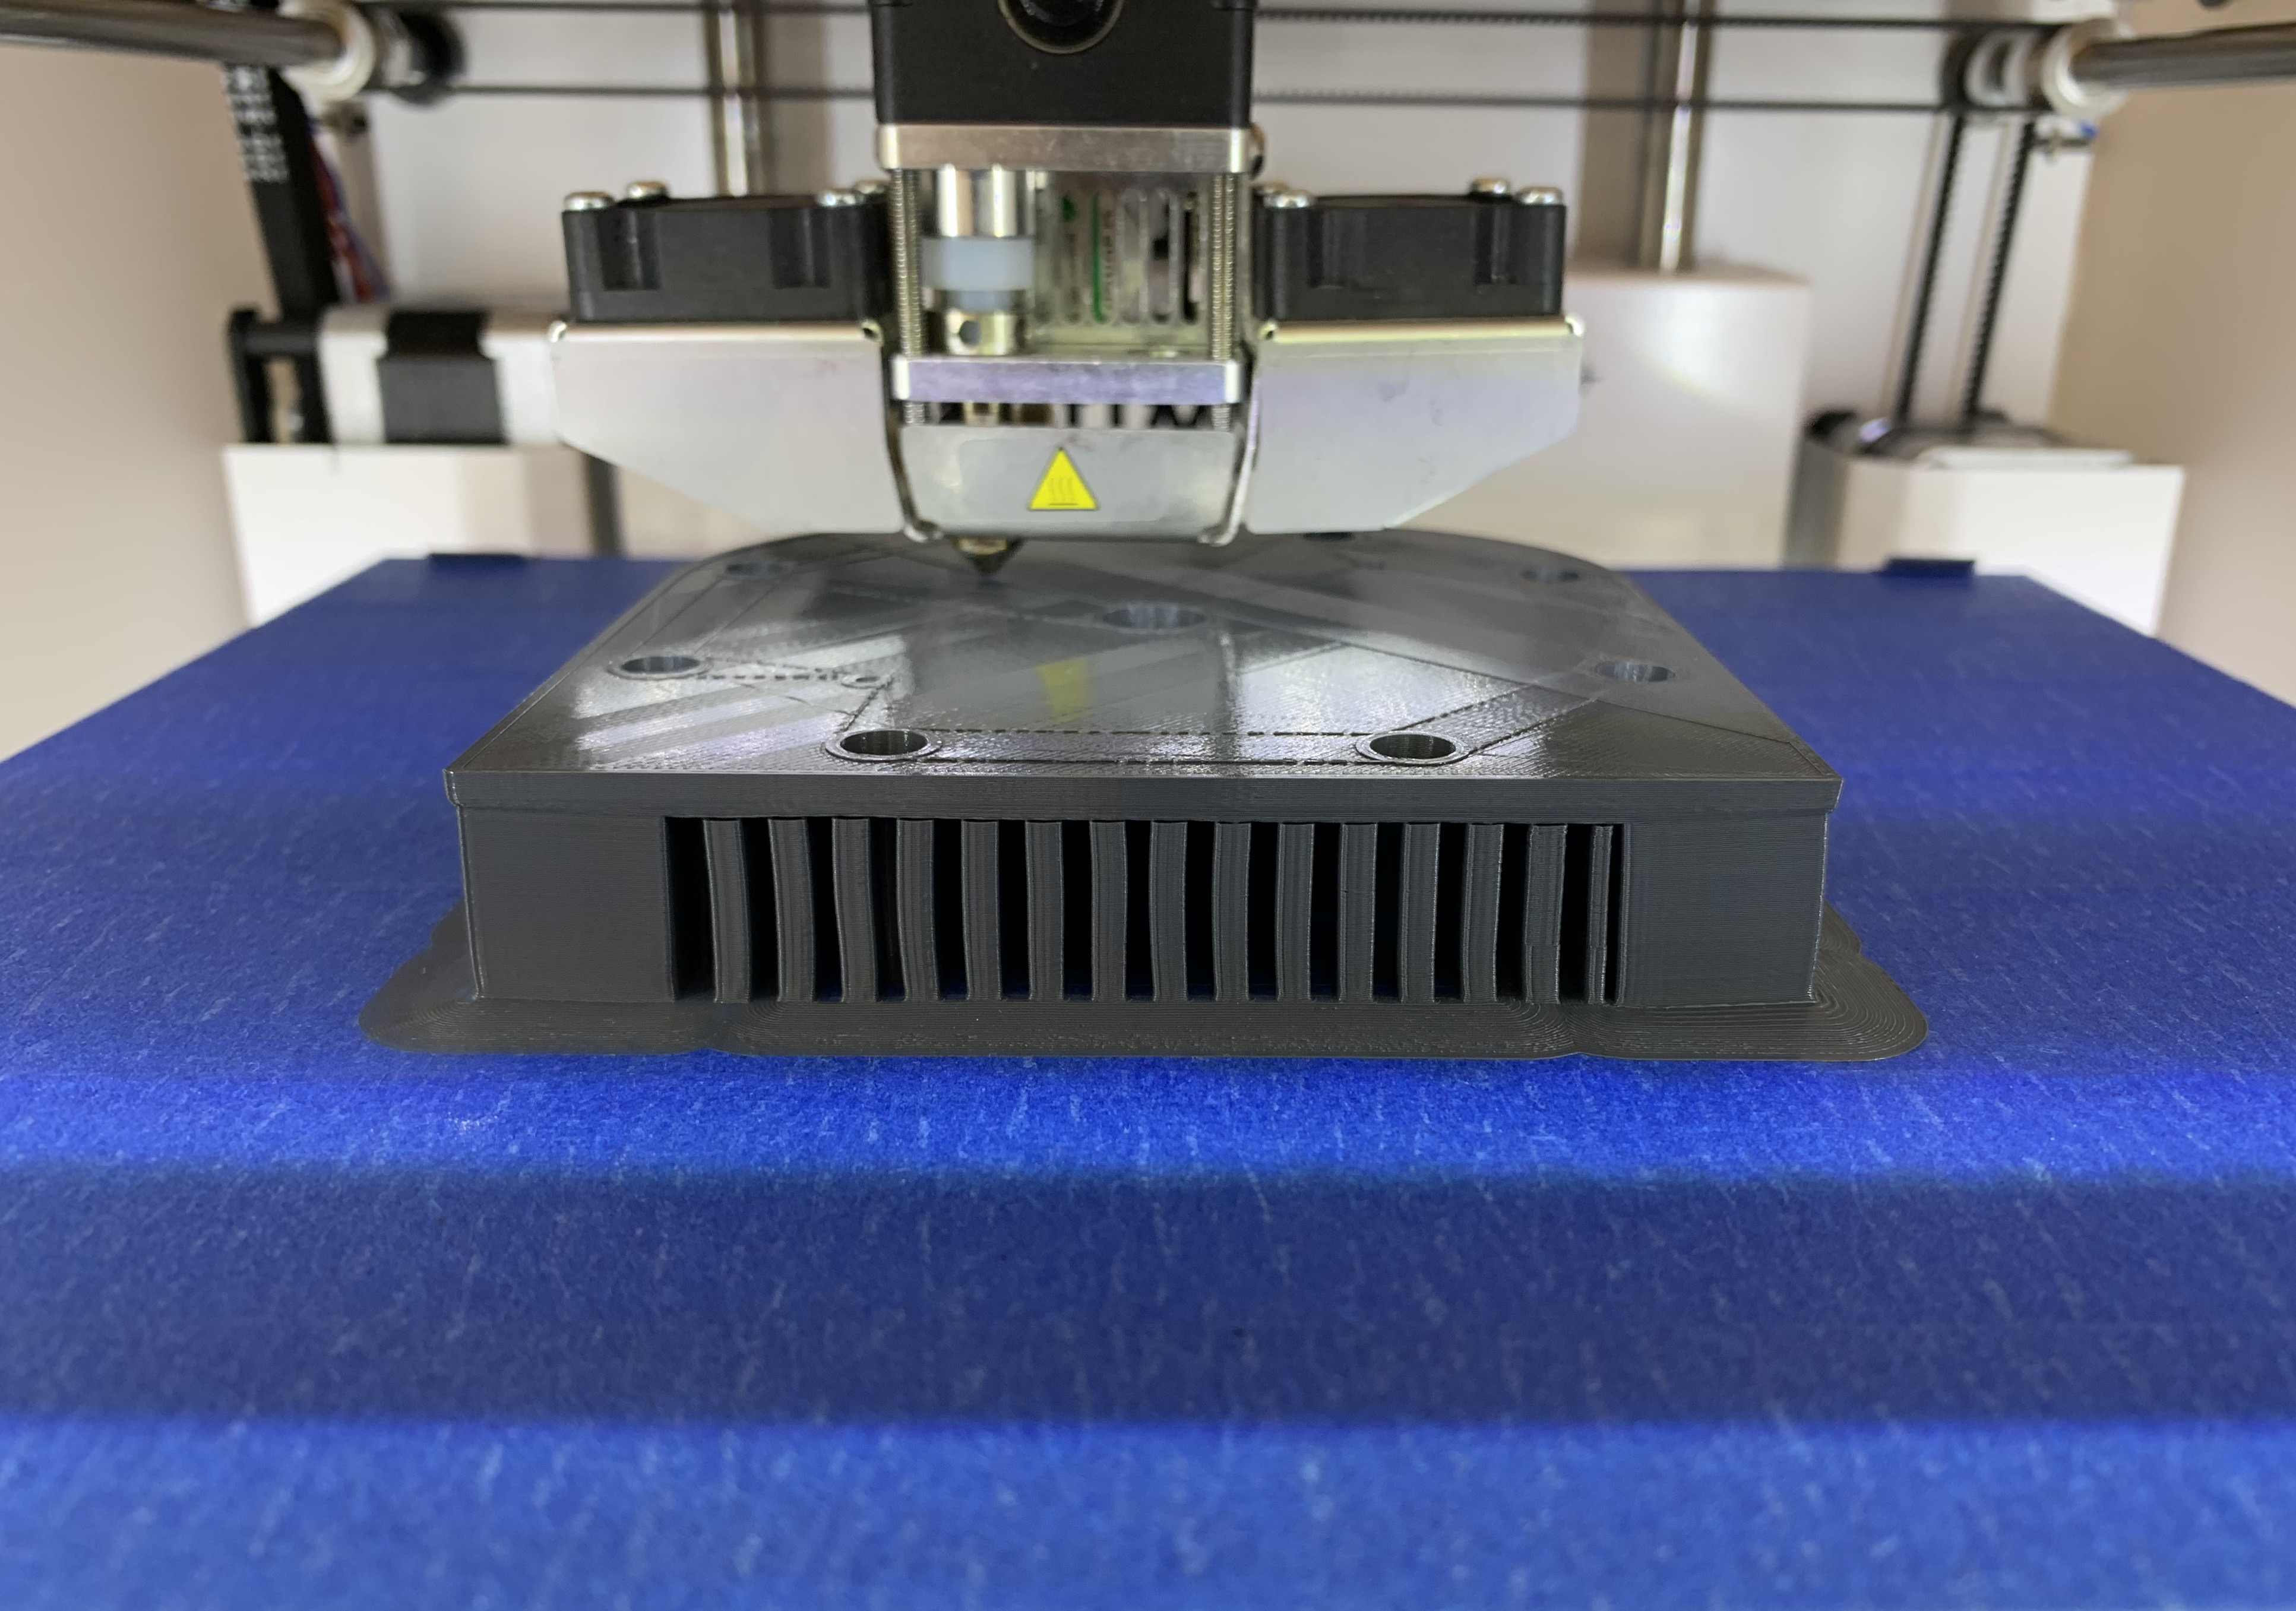
\includegraphics[width=0.6\textwidth]{DIV./Bilder/FinalPrint.jpg}
    \caption{Oxygen side being printed}
    \label{fig:Housingprint}
\end{figure}

\section{Assembling the fuel cell}

\subsection{Assembly with nickel foam gas diffusion layer}

When assembling the fuel cell we started by putting a double layer of Parafilm, PM-992, around the edges PEMFC housing to create a gas seal to make sure that no gas could escape. We also added a metal plate to create electrodes, for easy current collection. To allow the gas to get in front of the metal plate the corners blocking the input and output of the gases was cut away. As you can see on figure \ref{fig:GasSealMetal}.

\begin{figure}[ht]
    \centering
    \begin{subfigure}[b]{0.3\textwidth}
        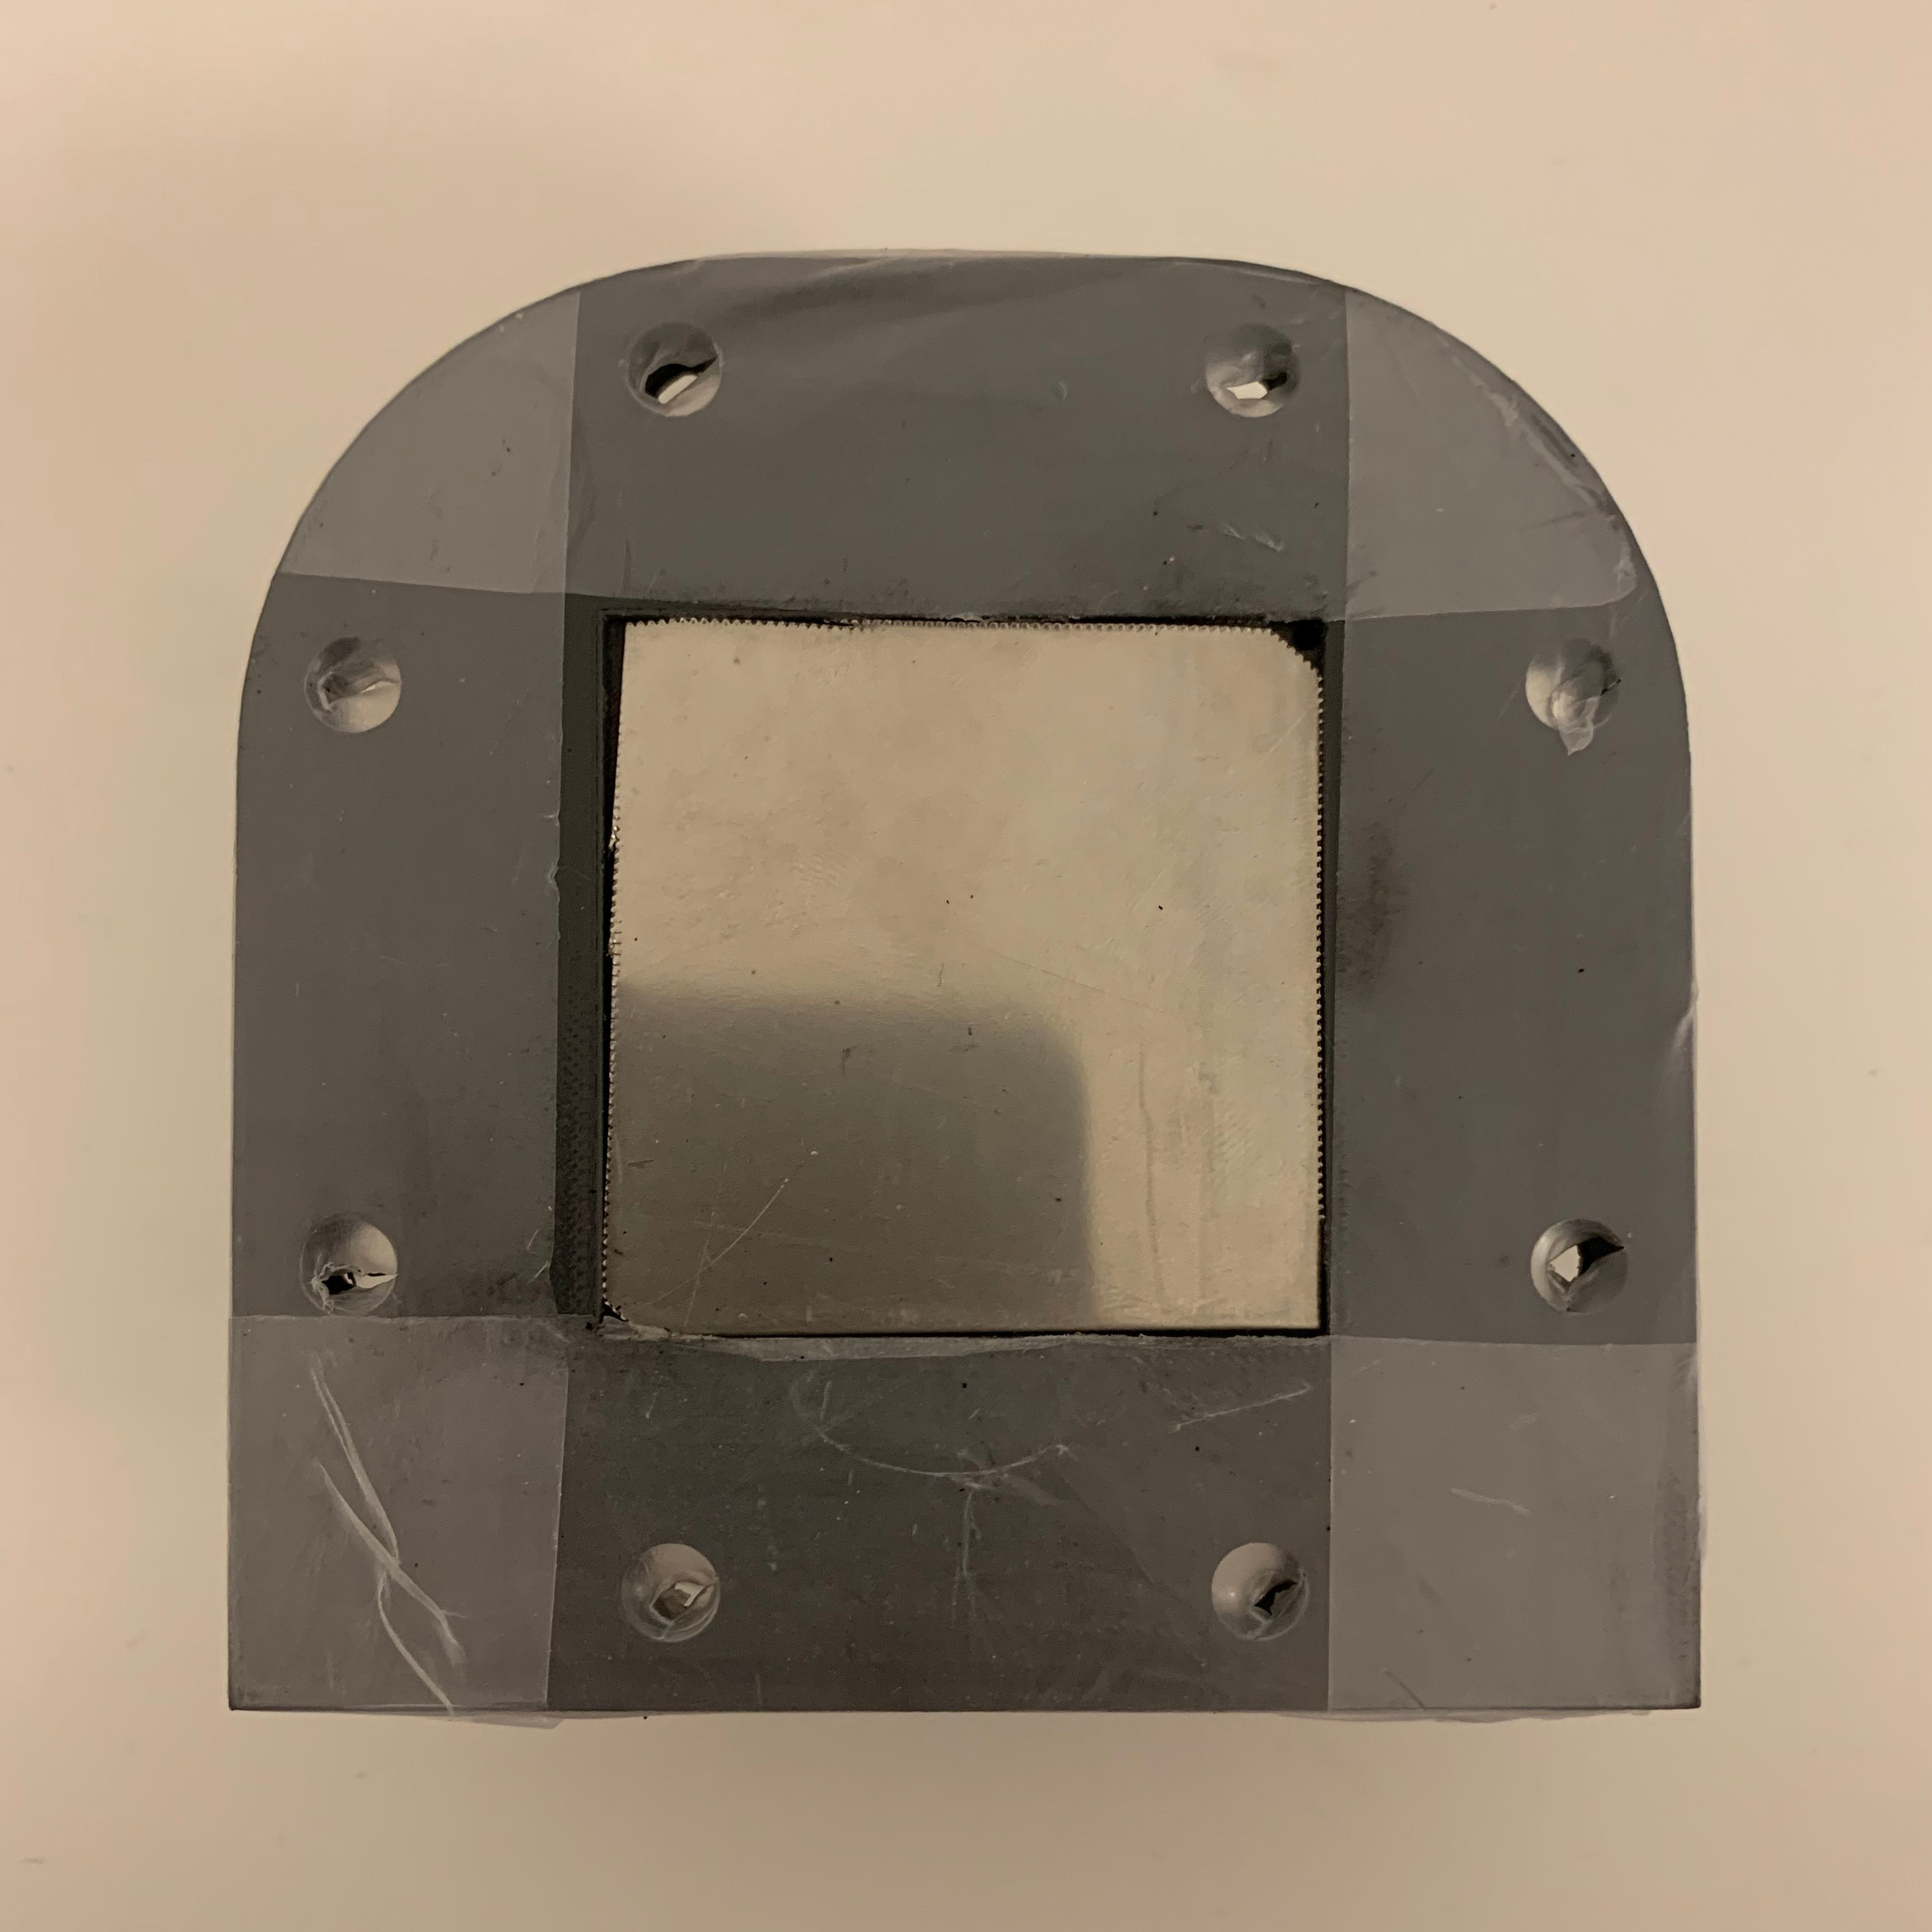
\includegraphics[width=\textwidth]{DIV./Bilder/Assembly/Ass1.jpg}
        \caption{Metalplate and Parafilm gas seal}
        \label{fig:GasSealMetal}
    \end{subfigure}
    ~ %add desired spacing between images, e. g. ~, \quad, \qquad, \hfill etc. 
      %(or a blank line to force the subfigure onto a new line)
    \begin{subfigure}[b]{0.3\textwidth}
        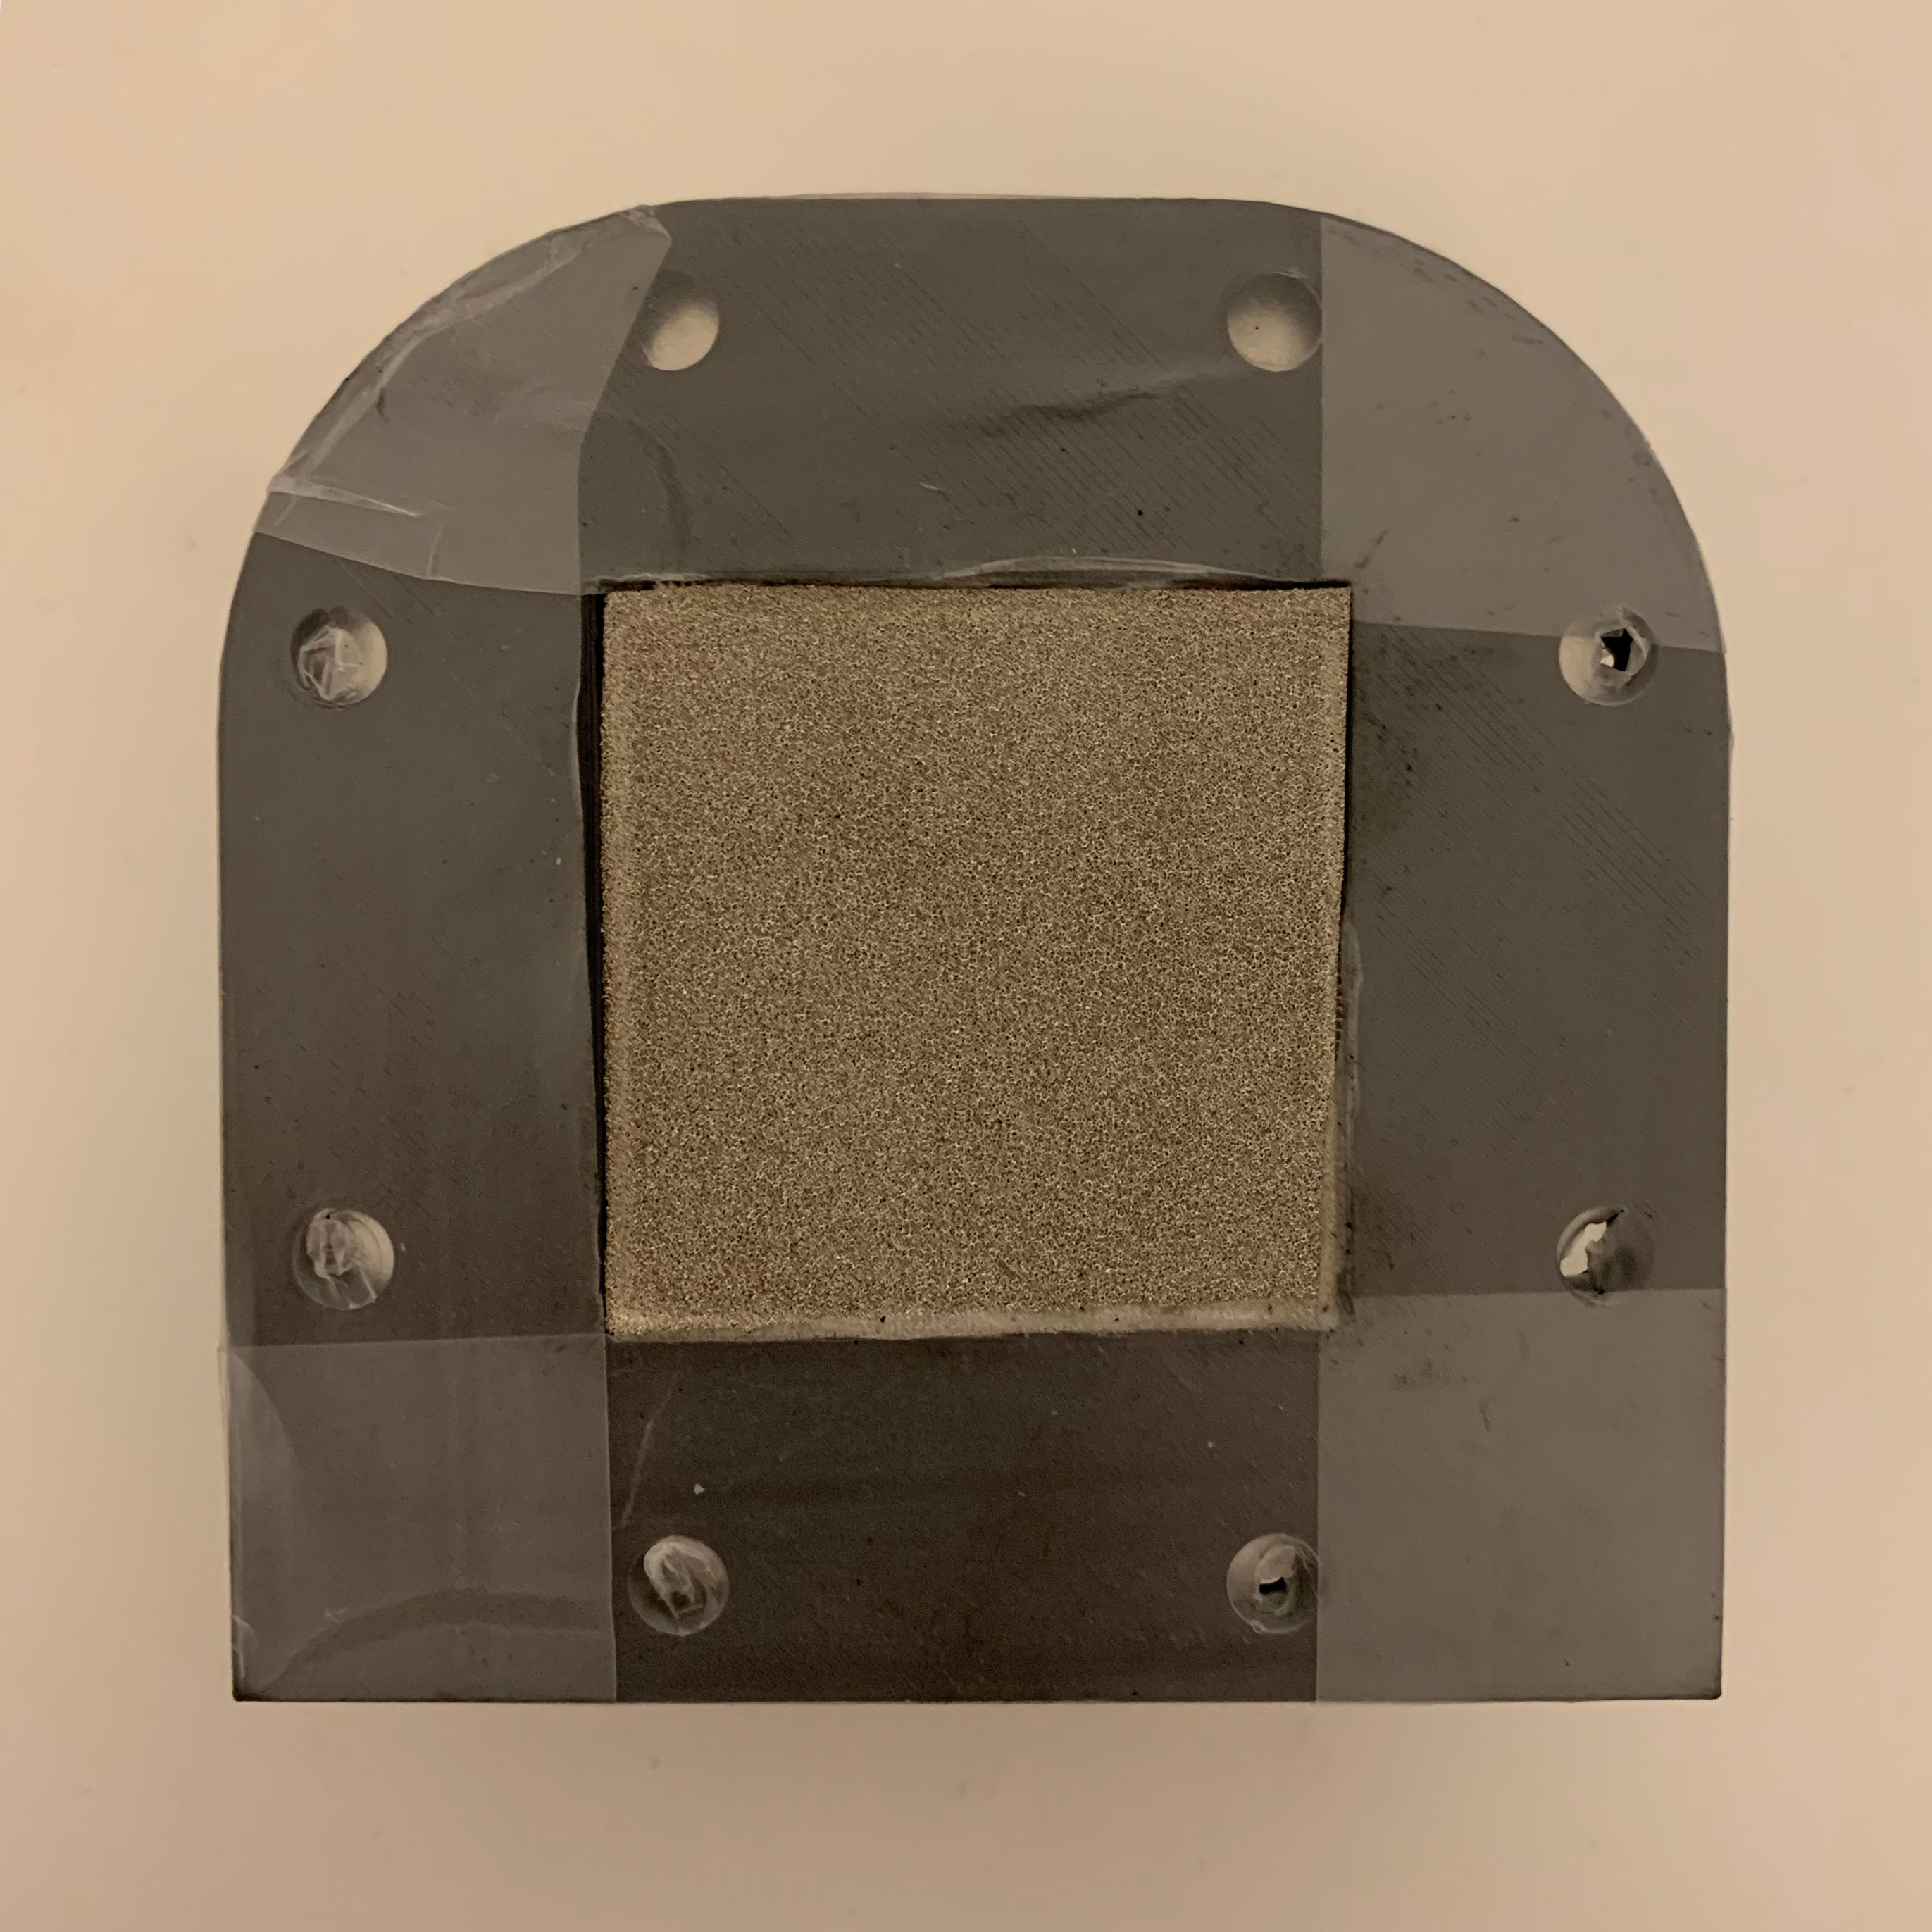
\includegraphics[width=\textwidth]{DIV./Bilder/Assembly/Ass2.jpg}
        \caption{Nickel foam gas diffusion layer}
        \label{fig:NickelFoam}
    \end{subfigure}
    ~ %add desired spacing between images, e. g. ~, \quad, \qquad, \hfill etc. 
    %(or a blank line to force the subfigure onto a new line)
    \begin{subfigure}[b]{0.3\textwidth}
        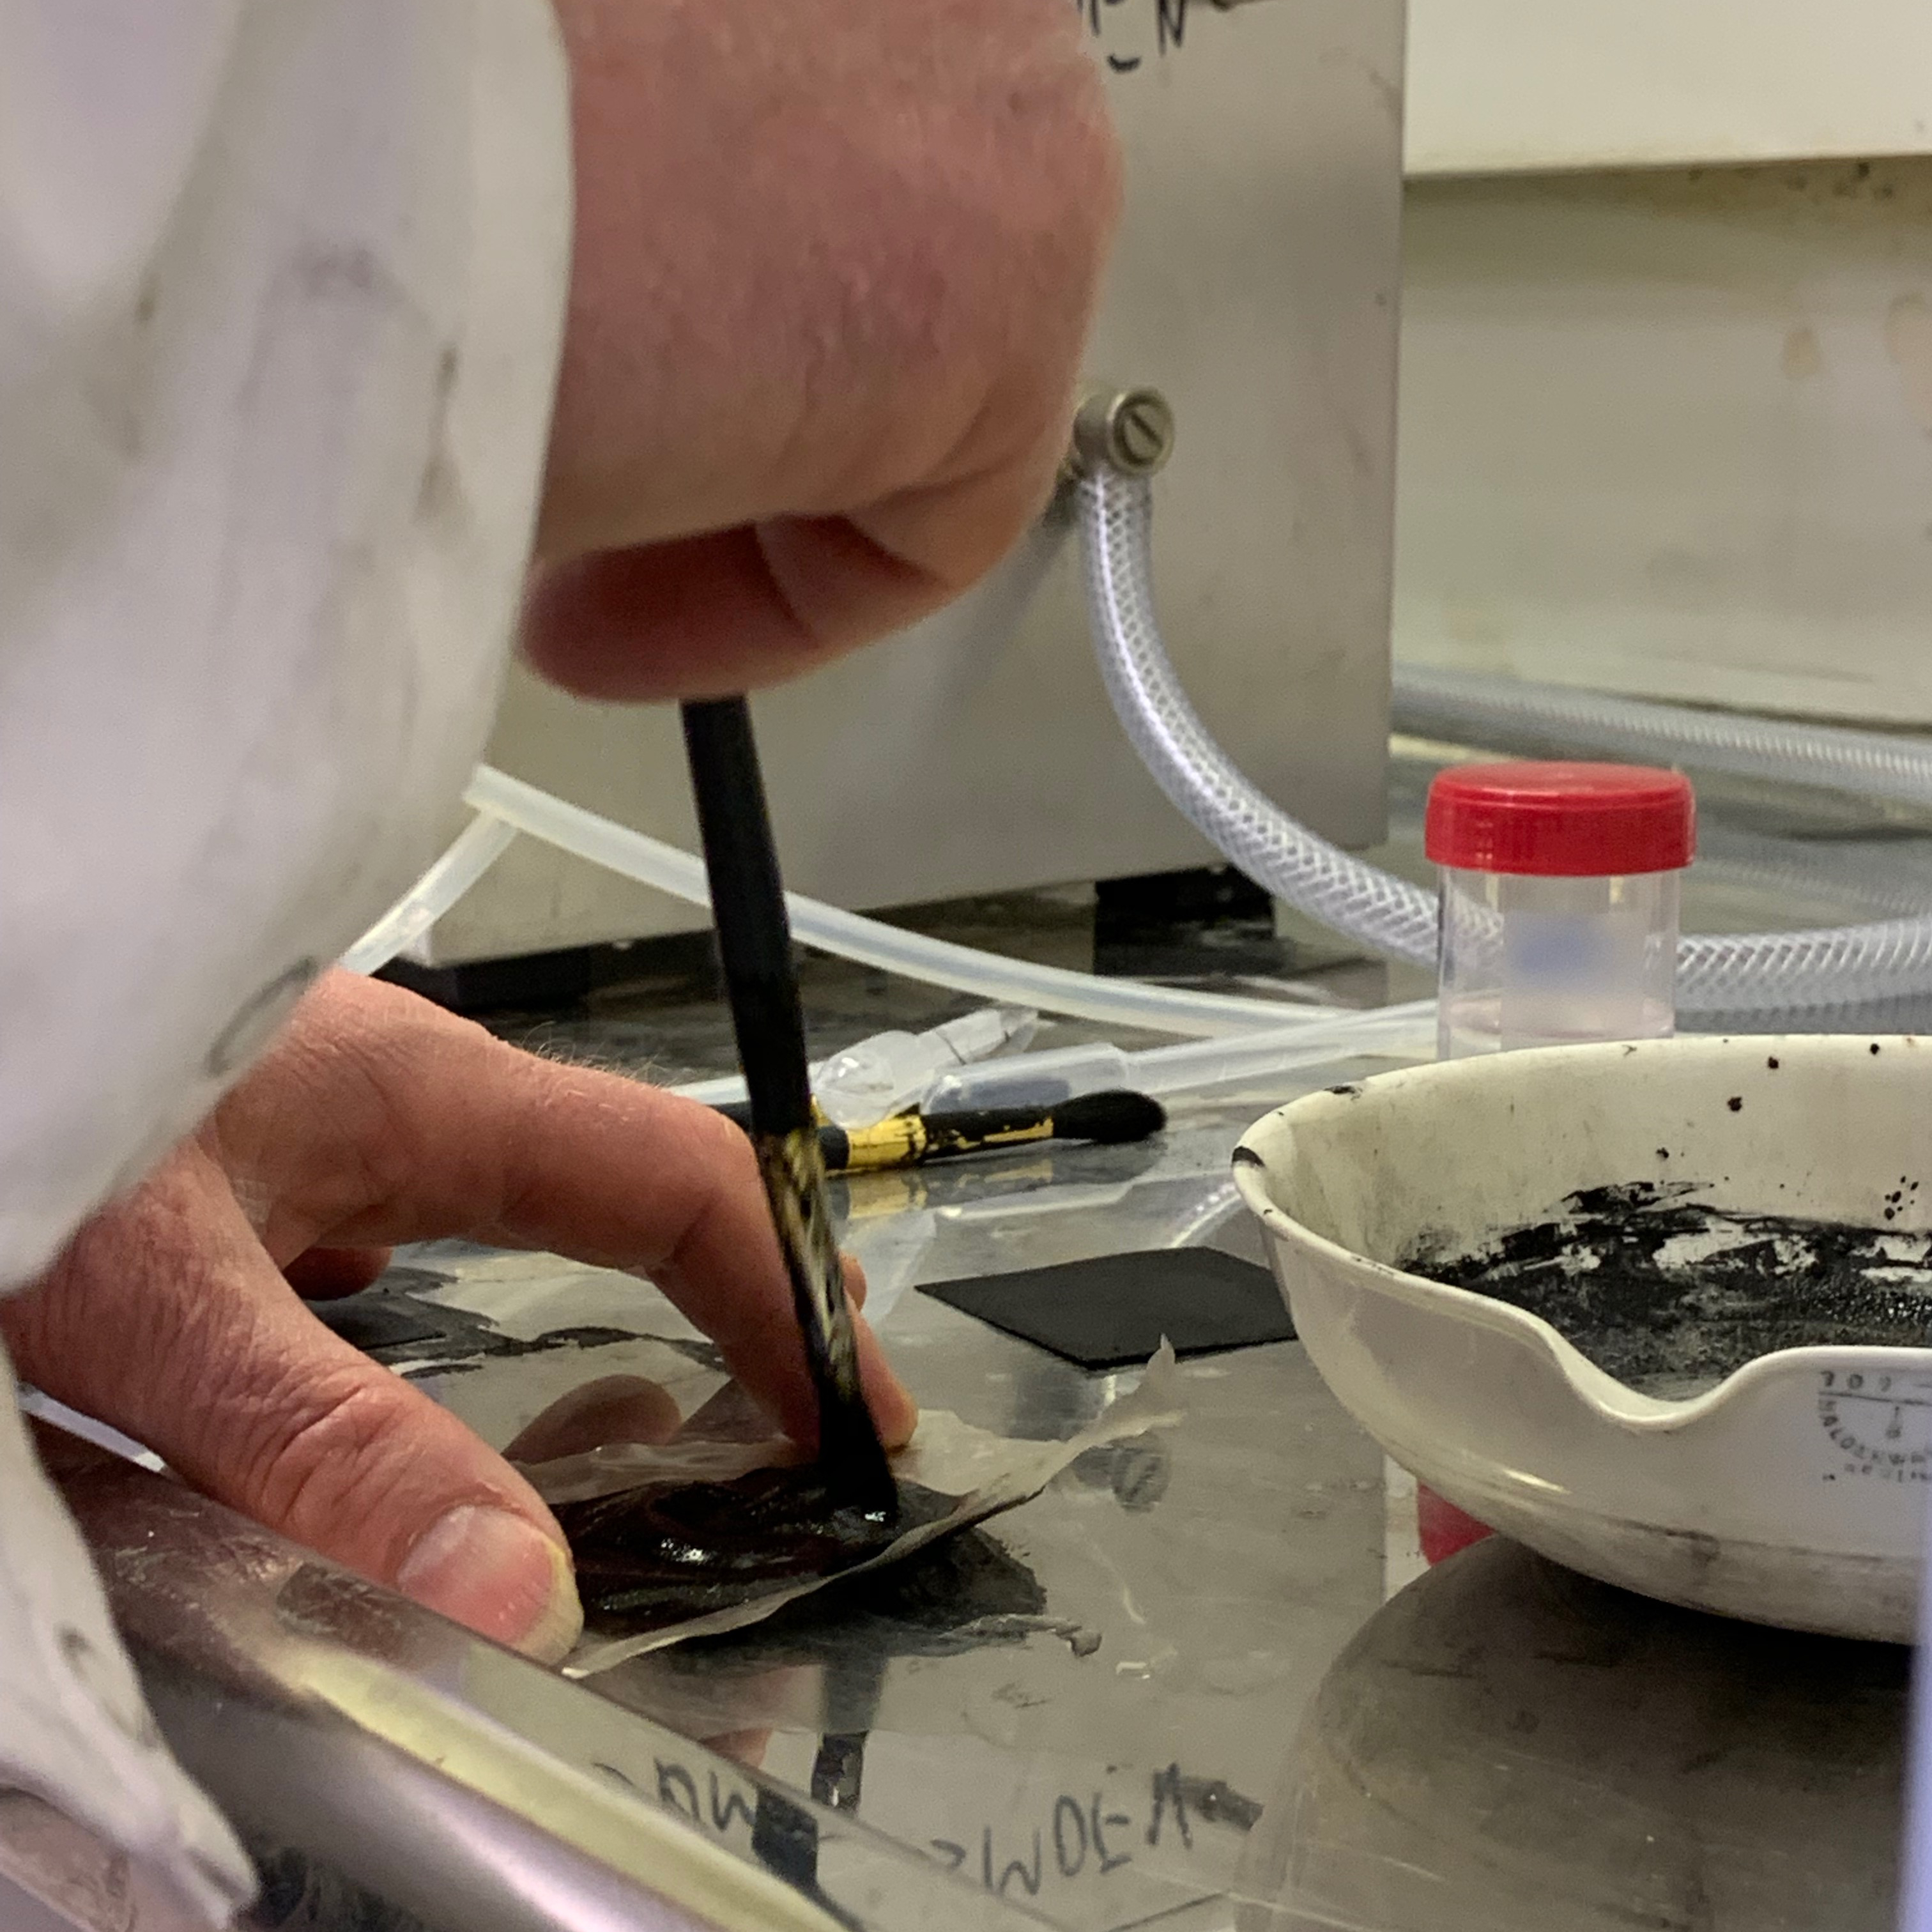
\includegraphics[width=\textwidth]{DIV./Bilder/Assembly/Ass3.jpg}
        \caption{Catalyst painted on membrane}
        \label{fig:CatalystPaint}
    \end{subfigure}
    \caption{Assembly of the metalplate, nickel foam and Parafilm}\label{fig:Assembly1}
\end{figure}

On top of the metal plate we placed the nickel foam. The nickel foam is used as a gas diffusion layer. The gas diffusion layer is used to spread the gas molecules better so that more reactions can happen at the same time. Due to the height of the nickel foam, and the little space in the PEMFC, the nickel foam was softly hammered flatter to make it fit. After flattening the nickel foam, it was cut to fit inside the fuel cell. This can be seen on figure \ref{fig:NickelFoam}.

The catalyst was then painted on the Nafion membrane and on the carbon electrodes. The carbon-platinum blend was mixed with isopropyl alcohol (IPA) to make the catalyst a thin liquid. This was done to make the catalyst easy to apply with a paintbrush, as seen on figure \ref{fig:CatalystPaint}. When left to dry the alcohol evaporated and left the catalyst on the membrane and on the carbon paper electrolytes. To quickly dry the membrane and the electrodes a heating plat was used. When the catalyst and the electrodes was dry they were added to the fuel cell. First an electrode was added then the membrane and on top of that the next electrode. This can be seen in figure \ref{fig:ElectrodeMembraneAssembly}


\begin{figure}[ht]
    \centering
    \begin{subfigure}[b]{0.3\textwidth}
        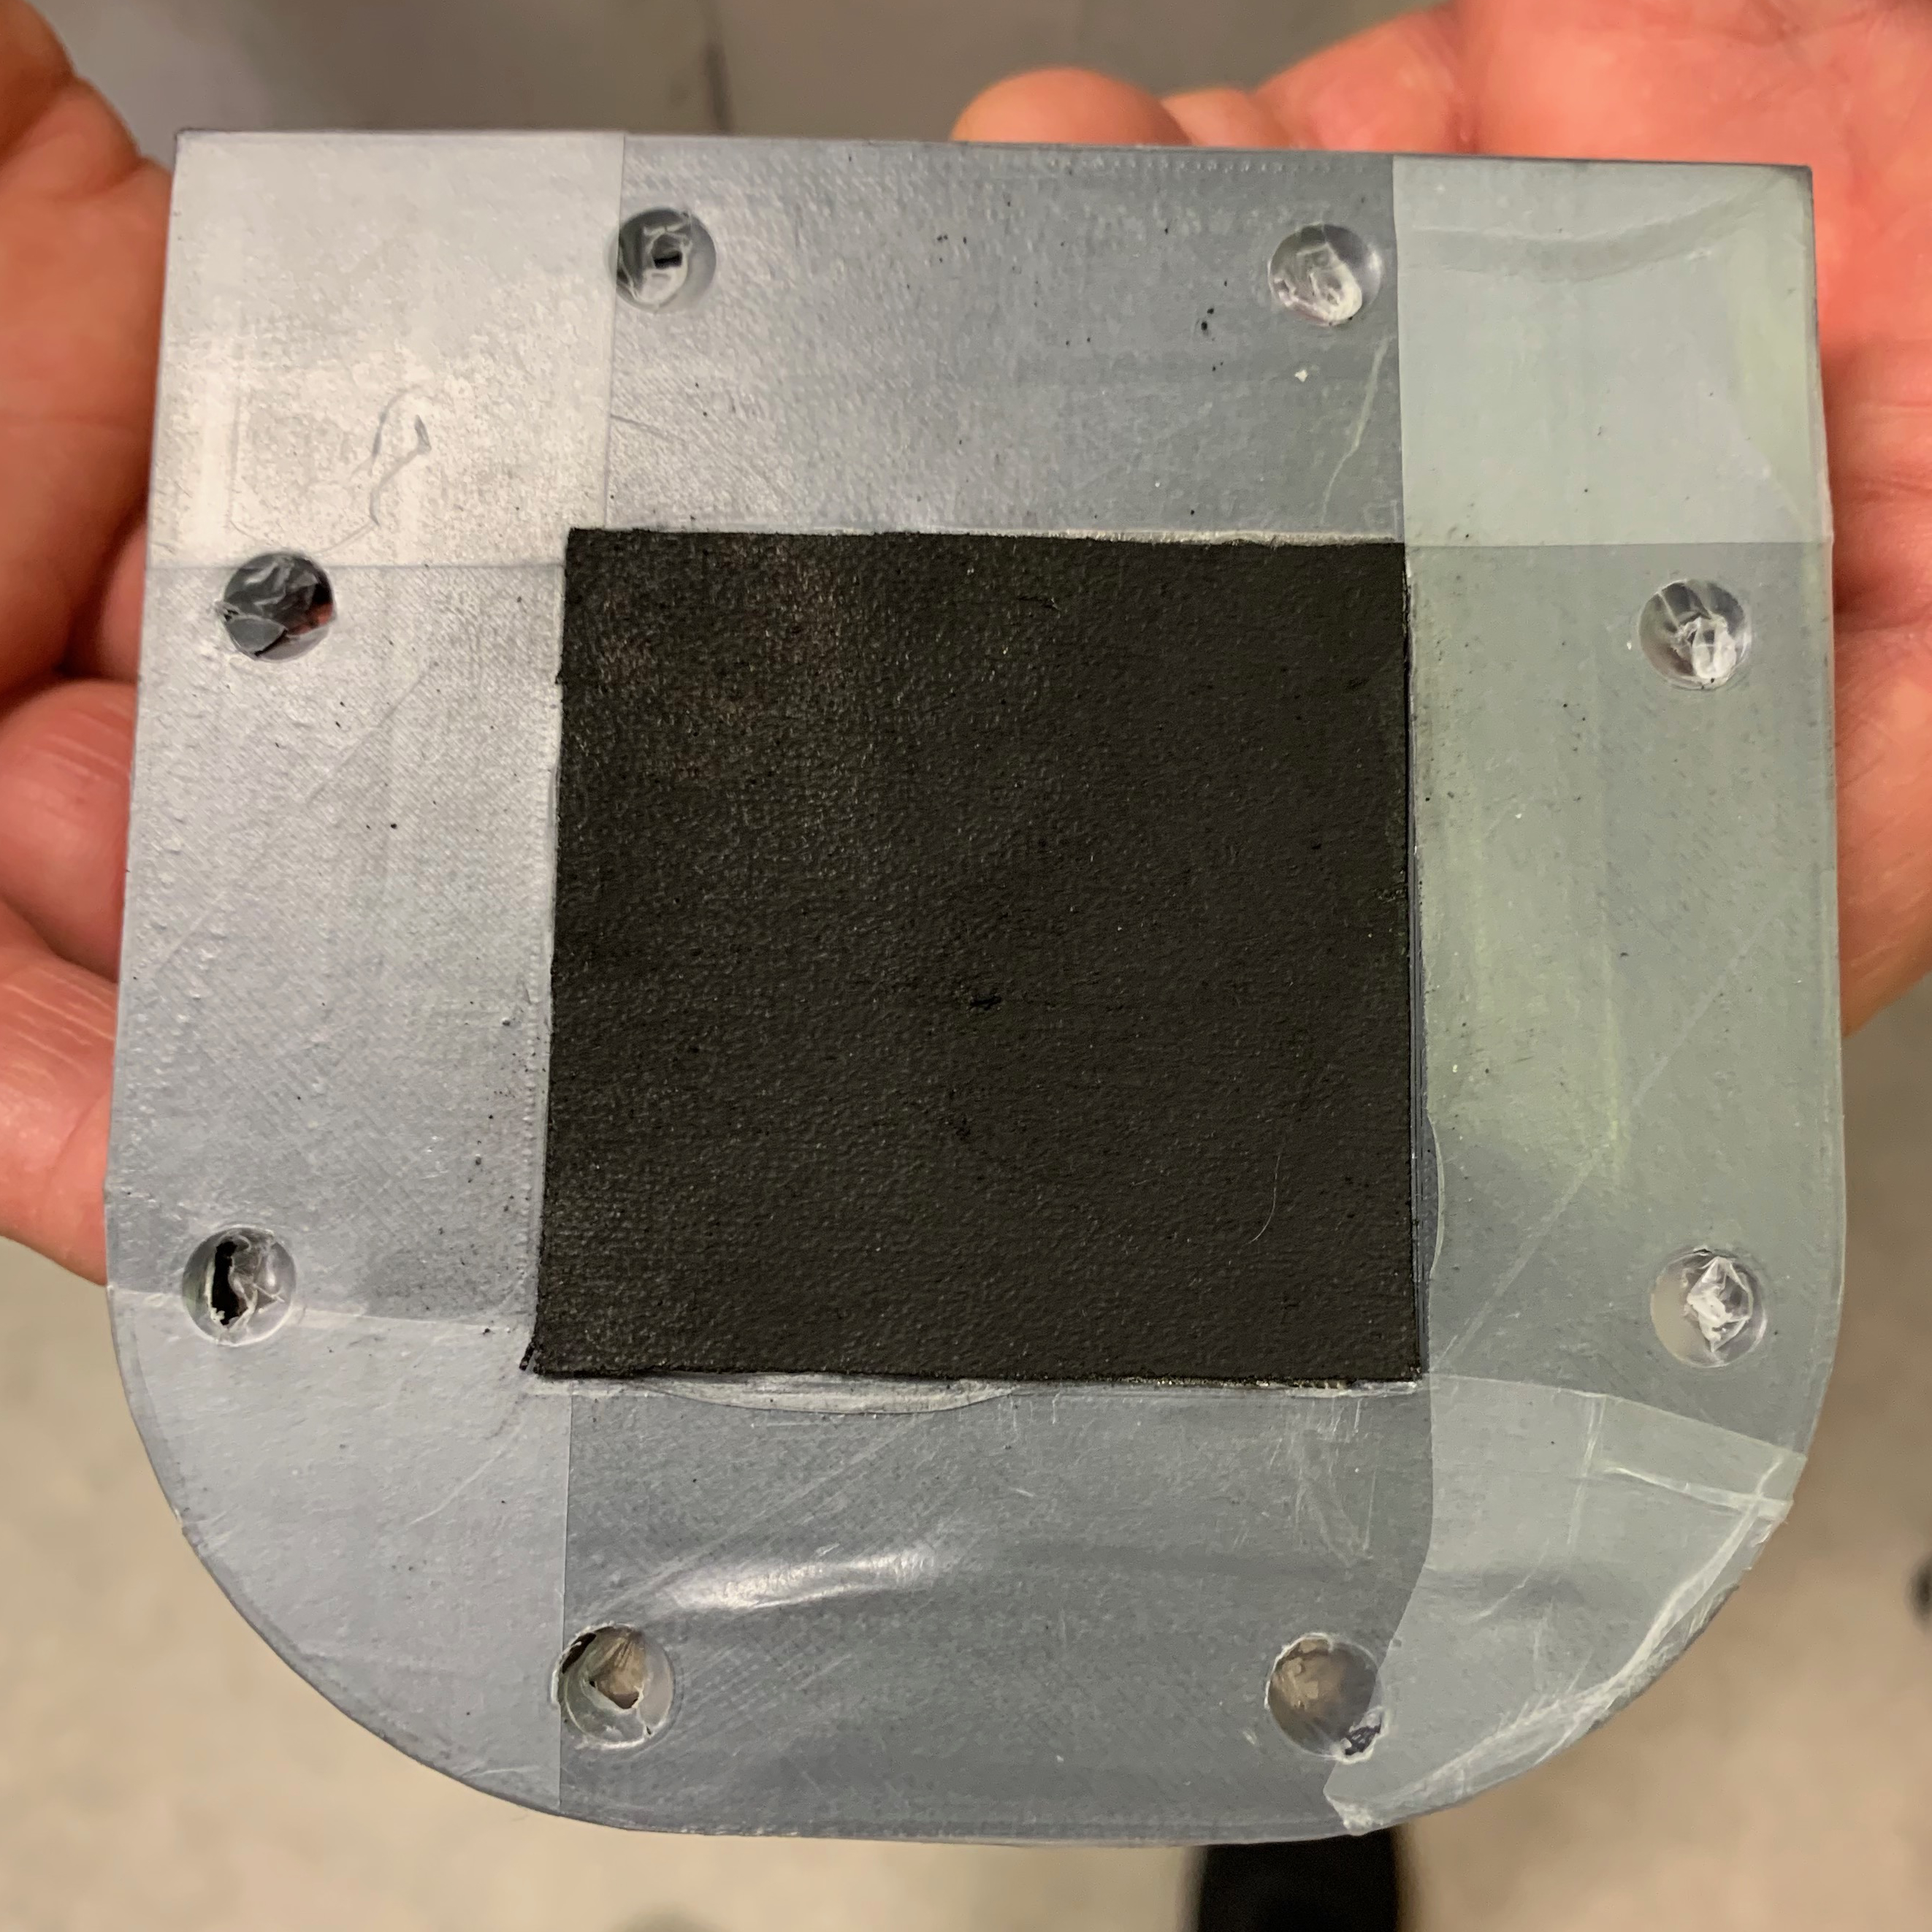
\includegraphics[width=\textwidth]{DIV./Bilder/Assembly/Ass4.jpg}
        \caption{The first electrolyte placed on top of the nickel foam}
        \label{fig:1Electrode}
    \end{subfigure}
    ~ %add desired spacing between images, e. g. ~, \quad, \qquad, \hfill etc. 
      %(or a blank line to force the subfigure onto a new line)
    \begin{subfigure}[b]{0.3\textwidth}
        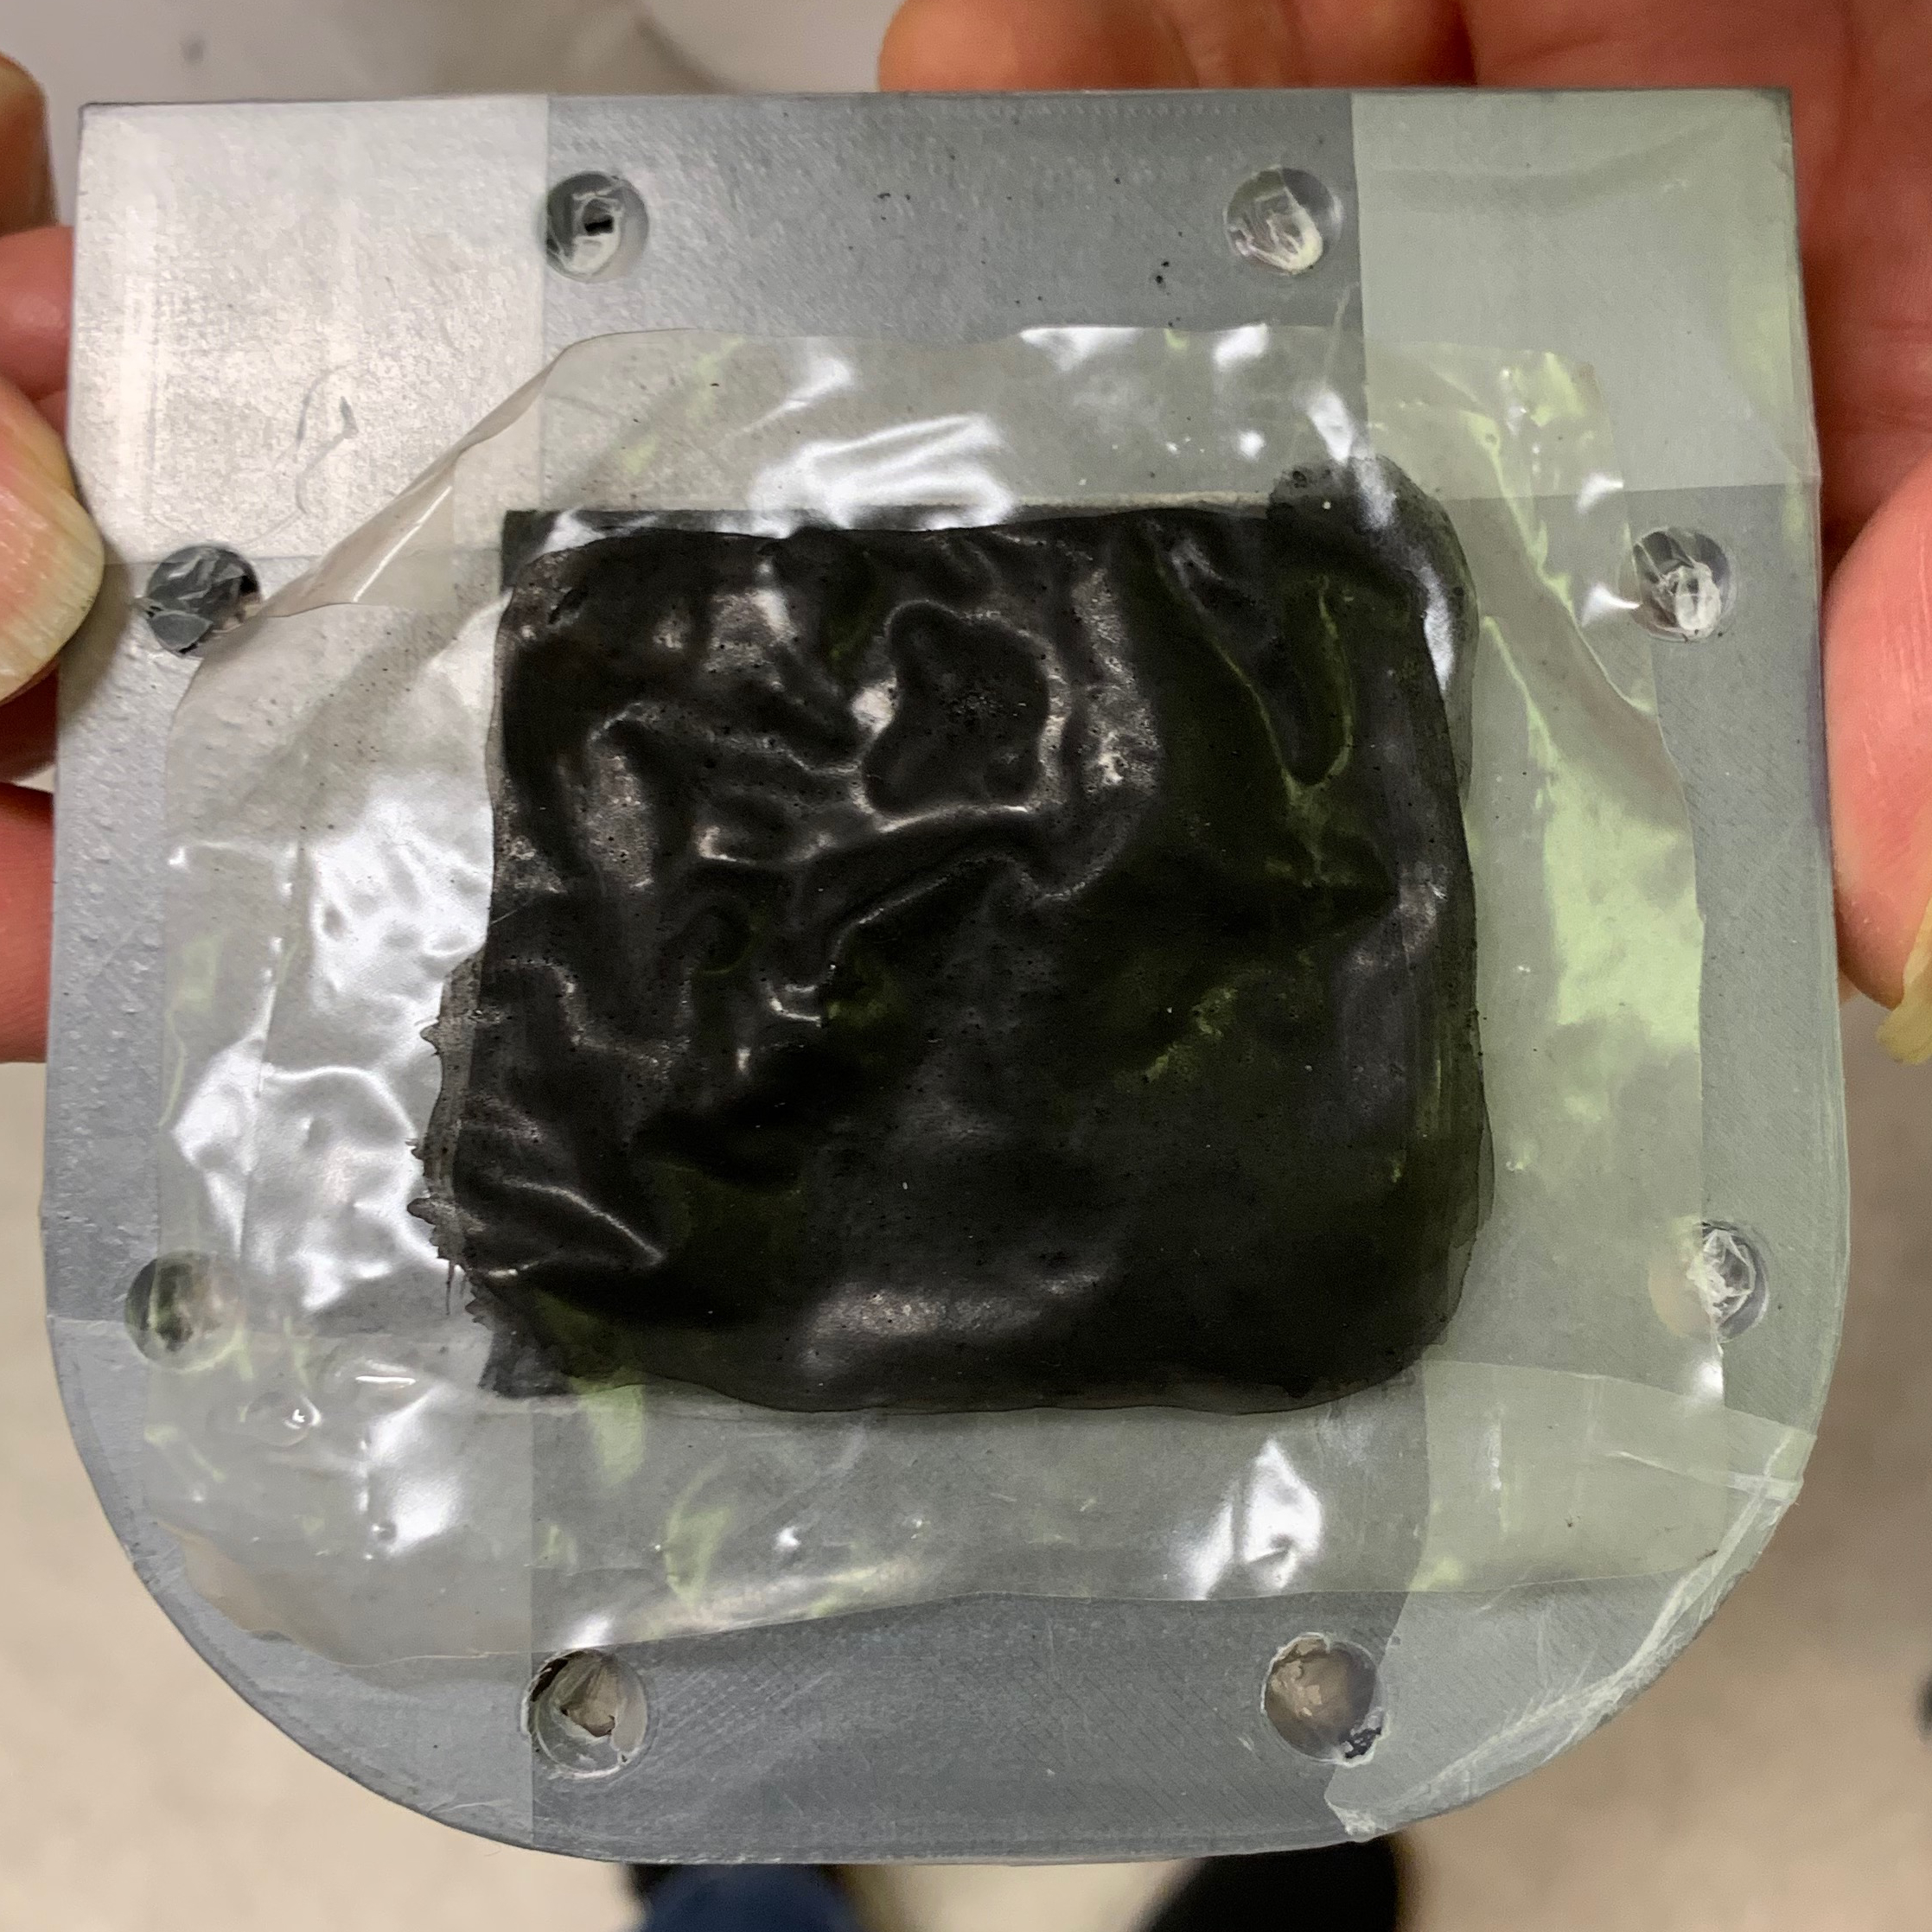
\includegraphics[width=\textwidth]{DIV./Bilder/Assembly/Ass5.jpg}
        \caption{The membrane inside the fuel cell}
        \label{fig:Membrane}
    \end{subfigure}
    ~ %add desired spacing between images, e. g. ~, \quad, \qquad, \hfill etc. 
    %(or a blank line to force the subfigure onto a new line)
    \begin{subfigure}[b]{0.3\textwidth}
        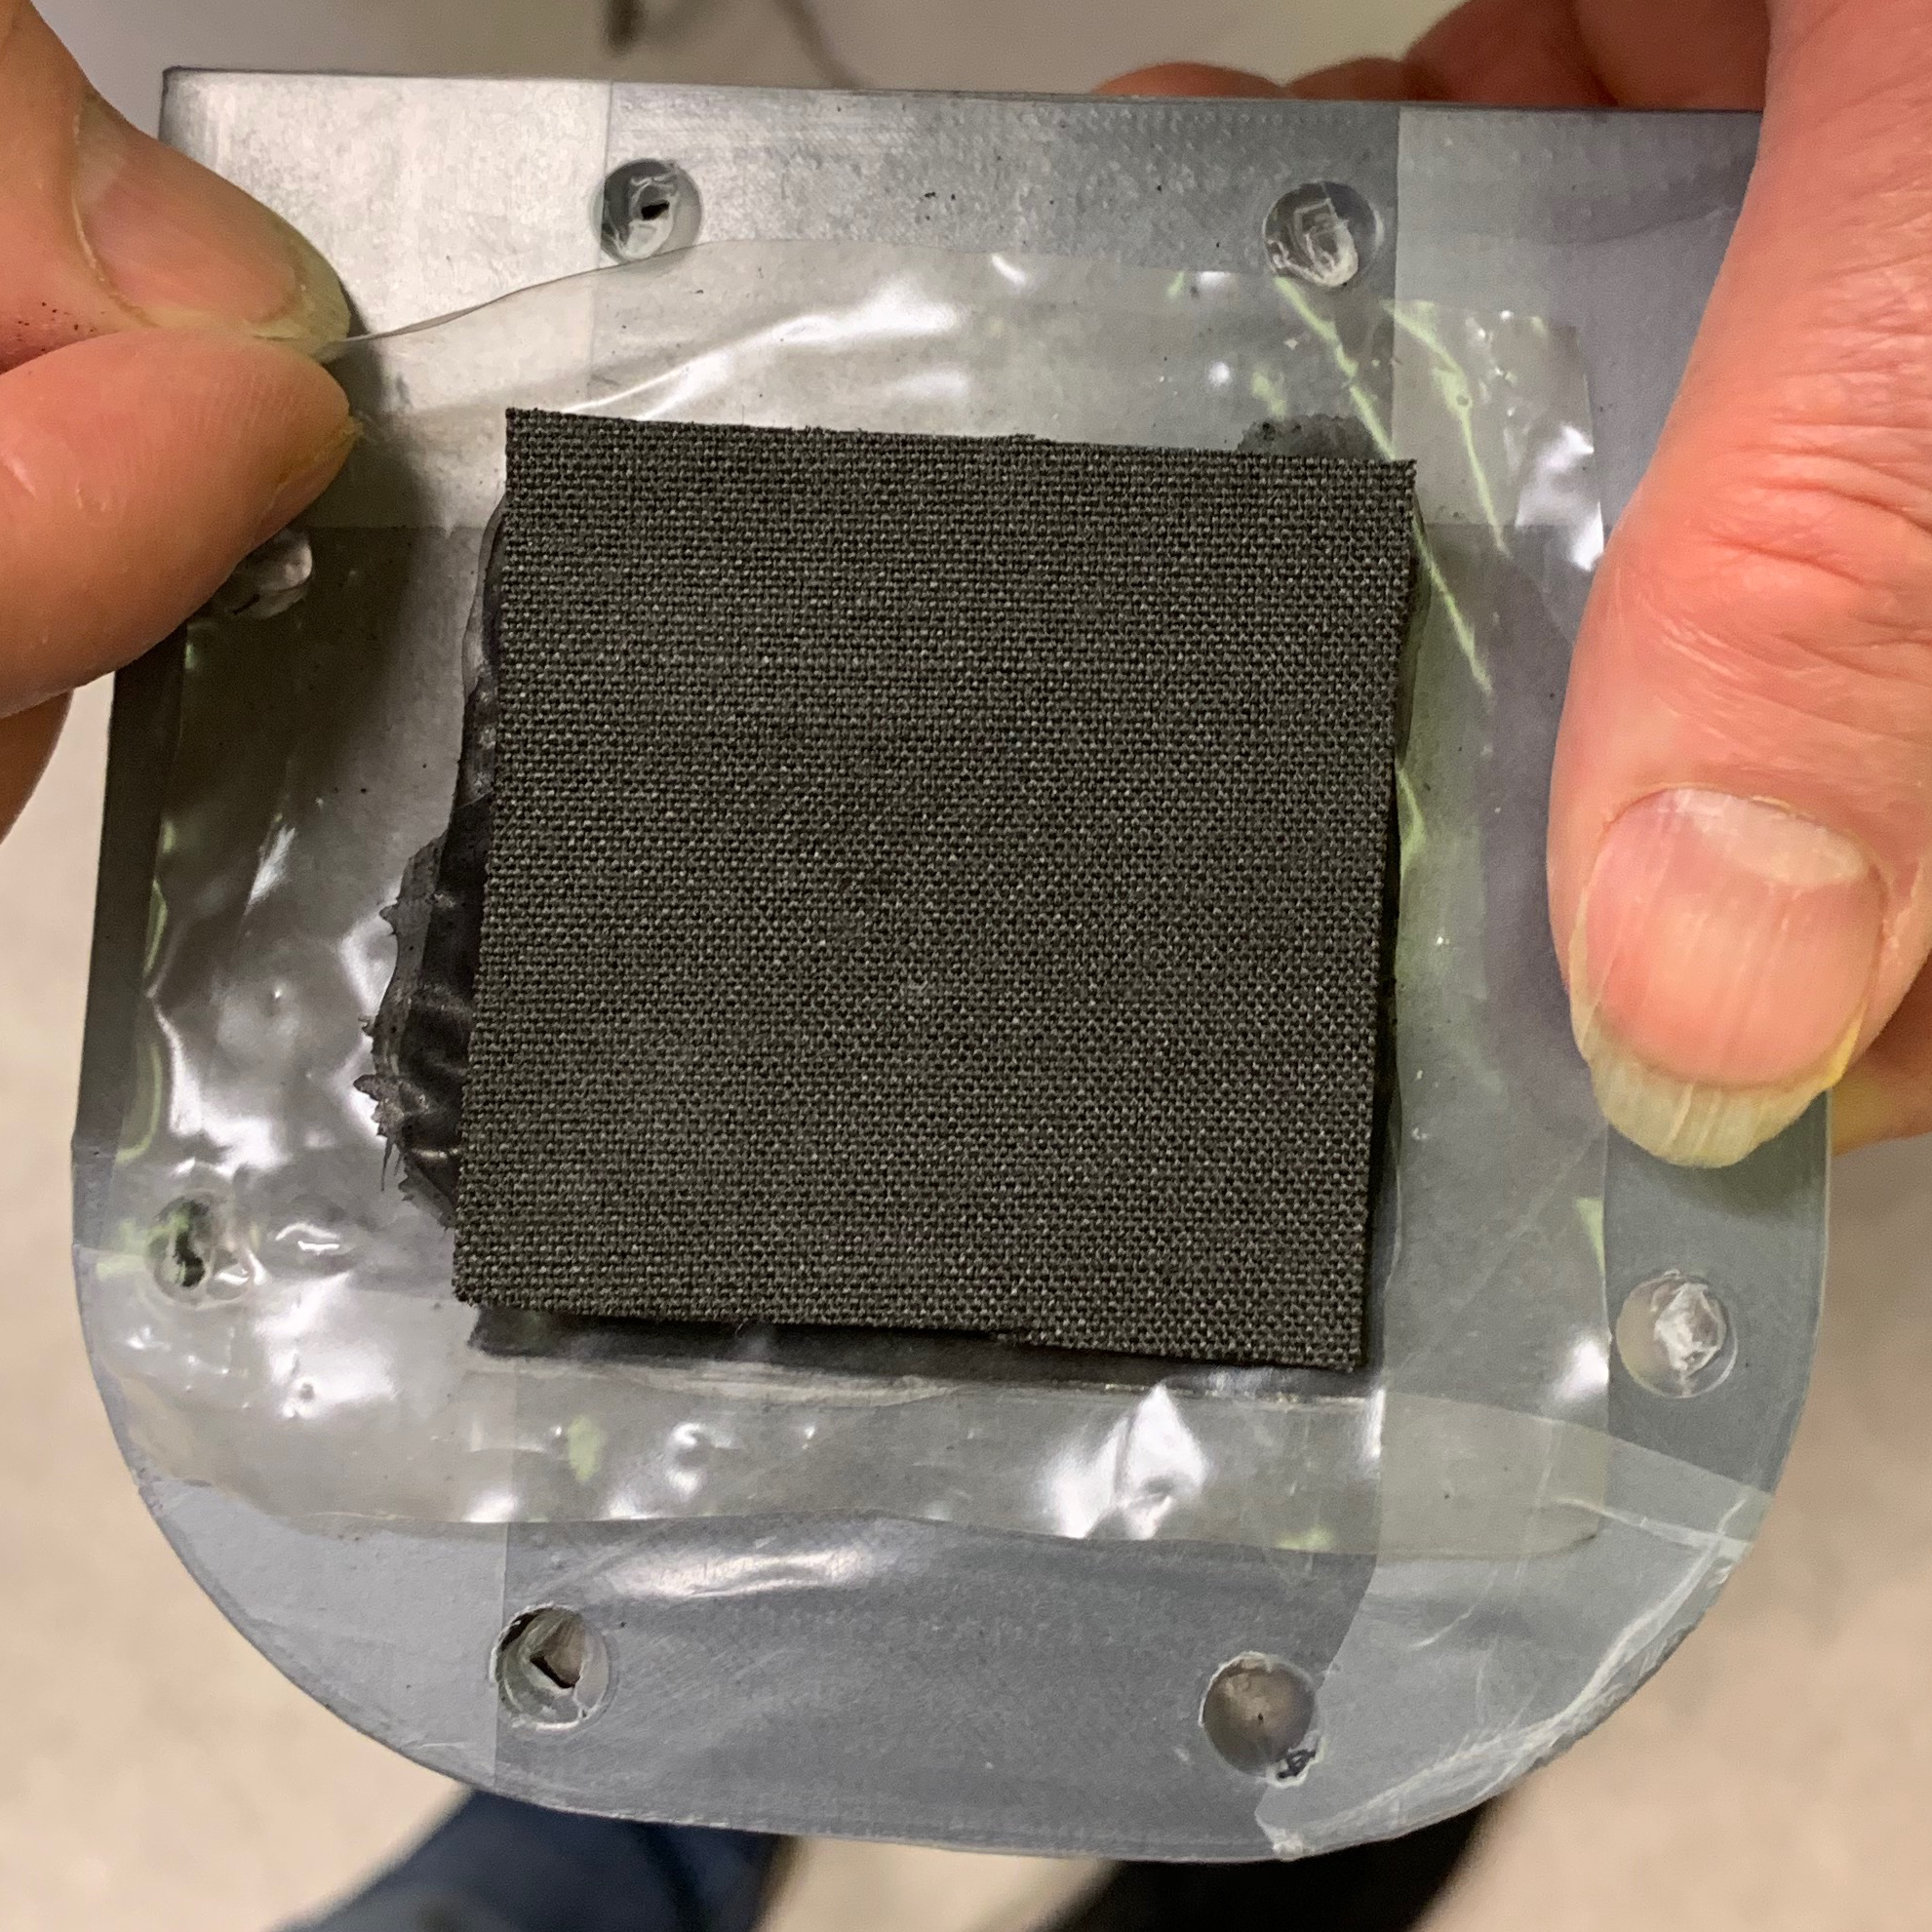
\includegraphics[width=\textwidth]{DIV./Bilder/Assembly/Ass6.jpg}
        \caption{The second electrode placed inside the fuel cell}
        \label{fig:2Electrode}
    \end{subfigure}
    \caption{Assembly of the electrodes and membrane}\label{fig:ElectrodeMembraneAssembly}
\end{figure}

The other side of the housing was then added and fastened together by eight M8 bolts and nuts. The bolts and nuts where tightened to make sure no gas could leak outside of the fuel cell. A bigger bolt, M12, was screwed in the middle of the fuel cell. We added Teflon tape on the end of the bolt to make sure it was an air tight fit. The M12 bolt was screwed in until it touched the metal plates inside the fuel cell. We could then use the M12 bolt to collect the voltage generated by the fuel cell. At the end a piece of tape was put on one side of the fuel cell to mark what side hydrogen should enter. The finished fuel cell can be seen on figure \ref{fig:FinishedFuelCell}.

\begin{figure}[ht]
    \centering
    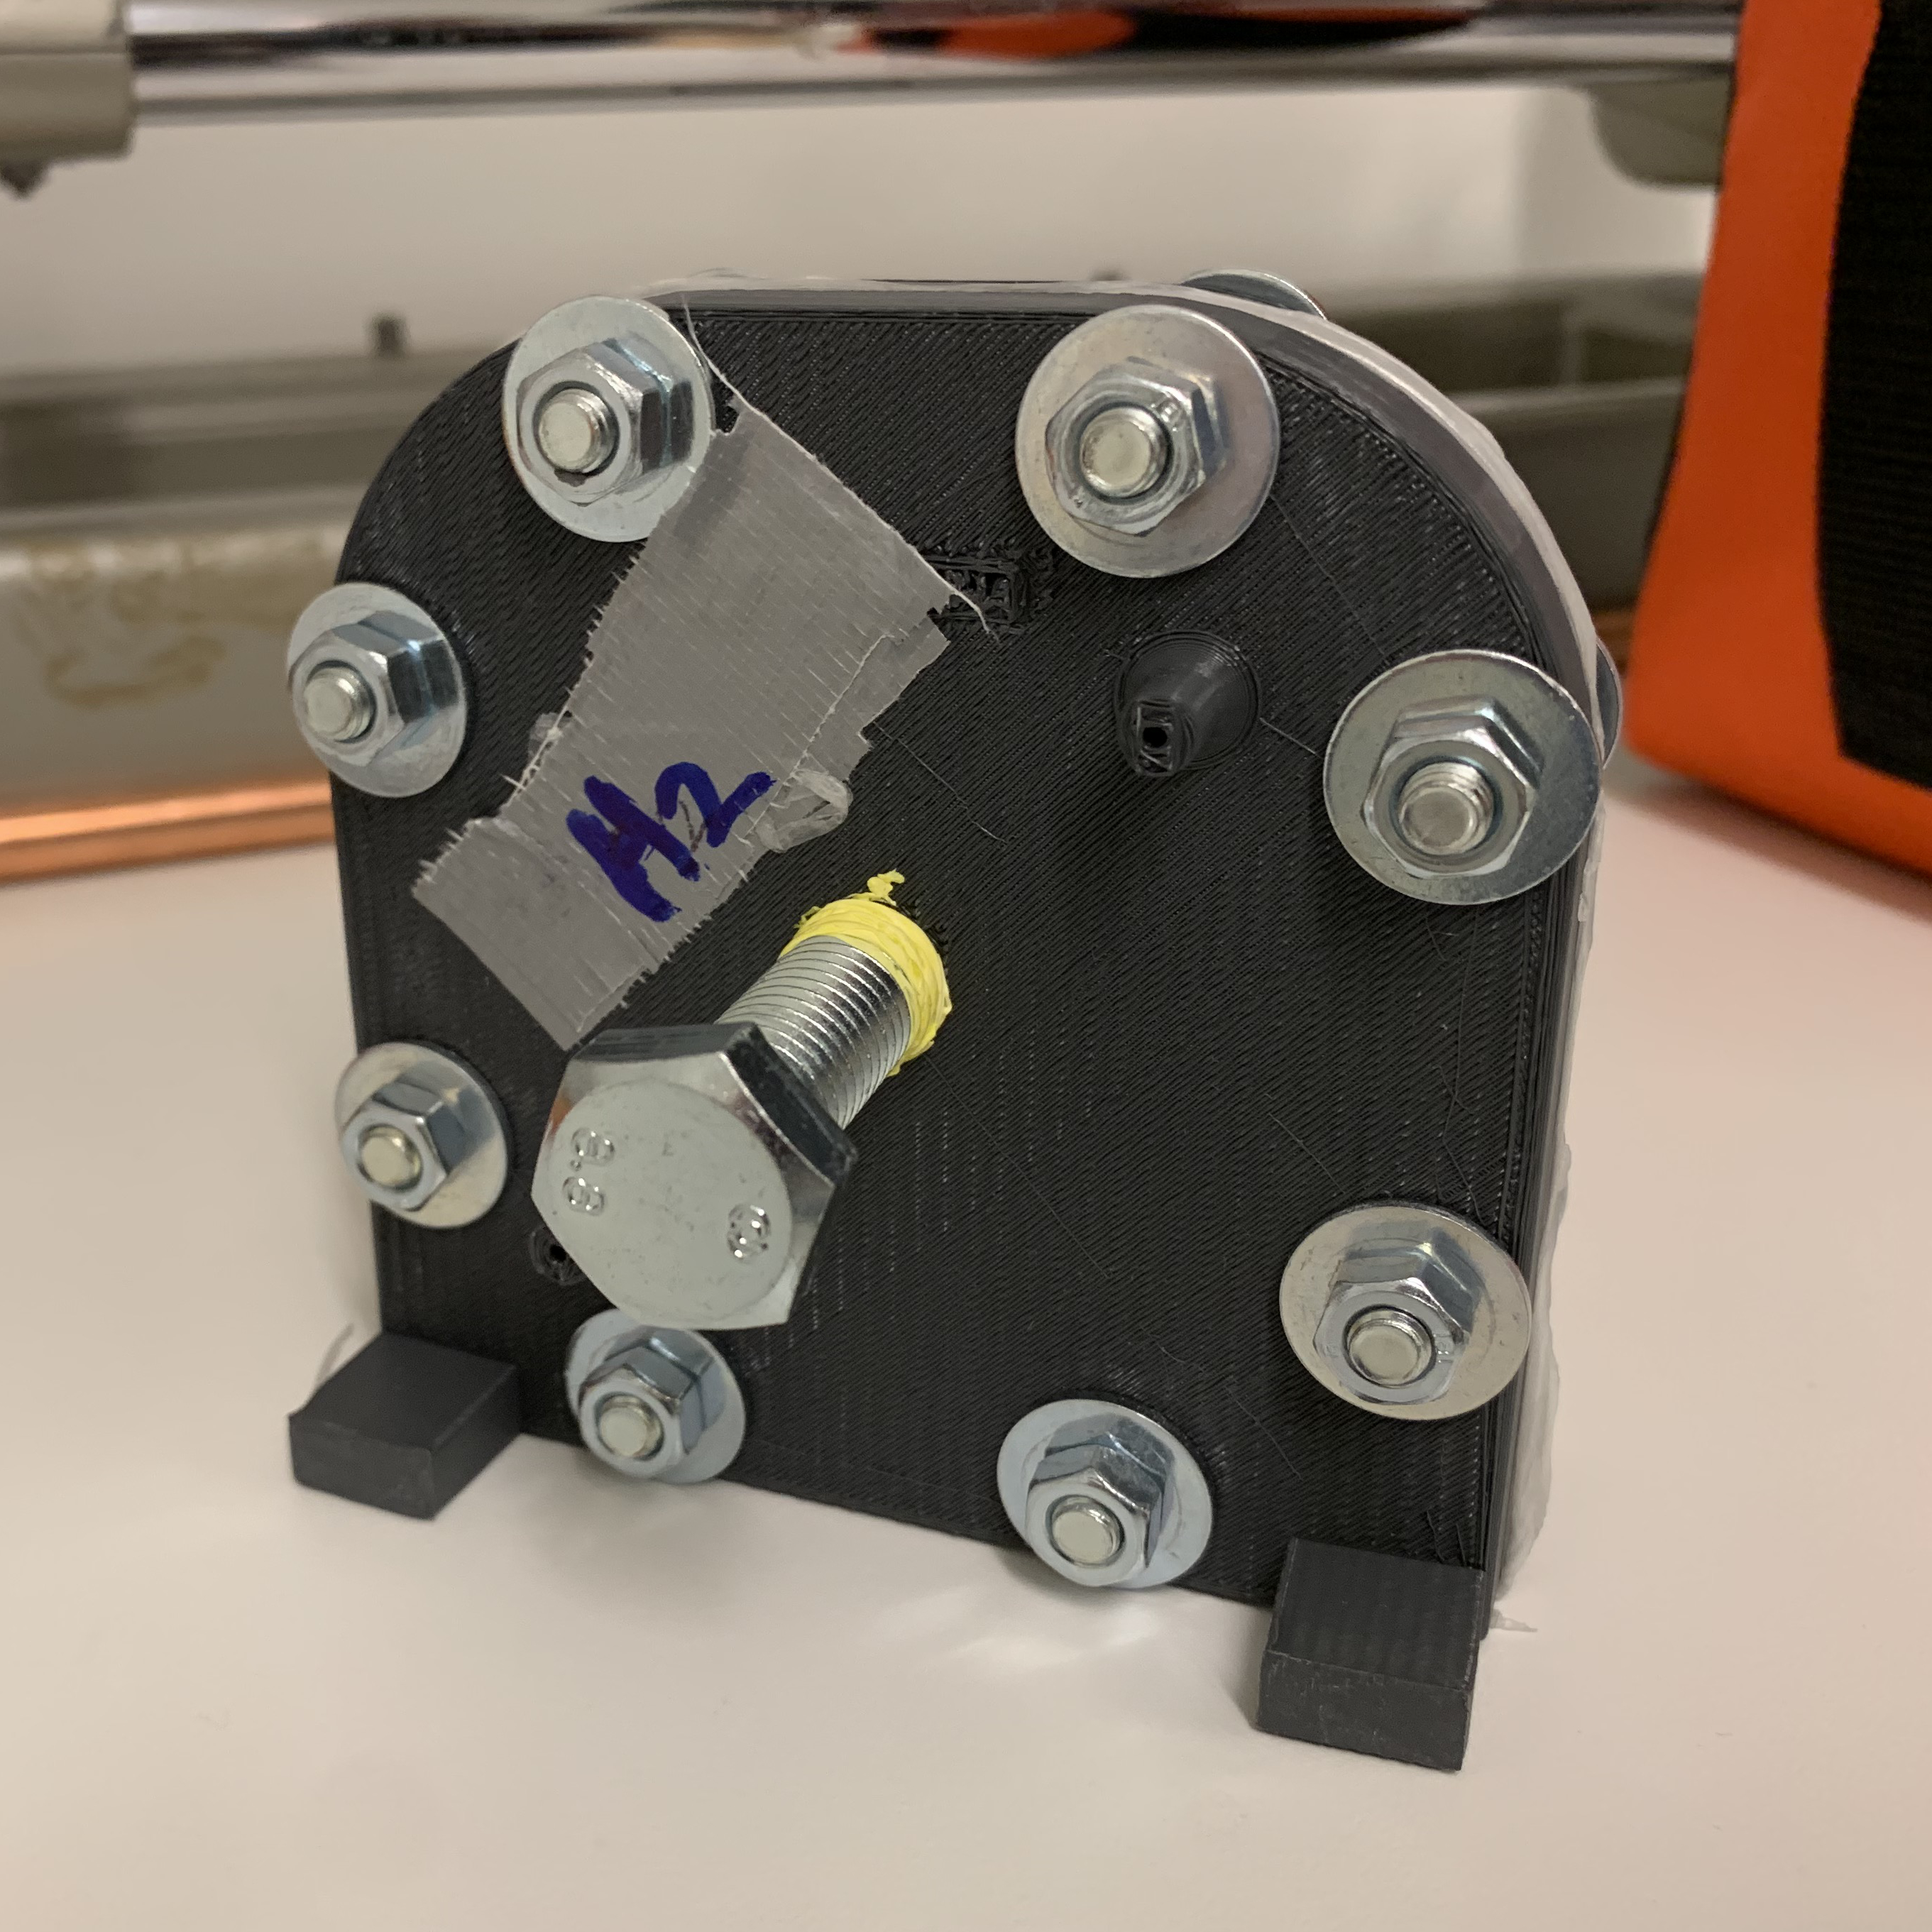
\includegraphics[width=0.4\textwidth]{DIV./Bilder/Assembly/Fuelcell.jpg}
    \caption{The fully assembled PEM fuel cell}
    \label{fig:FinishedFuelCell}
\end{figure}

\section{Testing}

The fuel cell was supplied with hydrogen from an outlet that was connected, through pipes, to hydrogen storage tanks. Oxygen was supplied through air that was pumped by an electric air-pump to create a continuous flow through the fuel cell. Both gasses were supply via tubes that was connected to the bottom tap on their respective sides of the fuel cell. Exit tubes were connected to the top taps while the other ends of the was placed in water, this way we could visually verify that there was a flow of gas. We connected the fuel cell to a load bank to easily be able to change between loads during our tests. Two voltmeters were used in the setup, one was placed to measure voltage over the fuel cell itself while the other was placed to measure voltage over the load.

We started the tests by measuring open circuit voltage, and proceeded by connecting a load-bank and measured the voltage over the first load step at 10.000 ohms. The load was decreased step by step while measuring voltage at each step.
 
We tested the fuel cell in four different setups. The first and second test was done using nickel foam as gas distribution layer inside of the fuel cell. The first test the fuel cell was dry, for the second test we filled the cell with water to soak the electrolyte. For the third and fourth tests, we took out the nickel distribution layer and repeated the testing process as was done in previous tests. This was done to test how well the fuel cell performed with the nickel foam distribution layer versus with only the carbon paper as a diffusion layer.

To make sure that the electrolyte was completely dry between the wet tests and the dry tests we placed it on a hotplate, on low heat, to make the water evaporate.

\begin{figure}[ht]
    \centering
    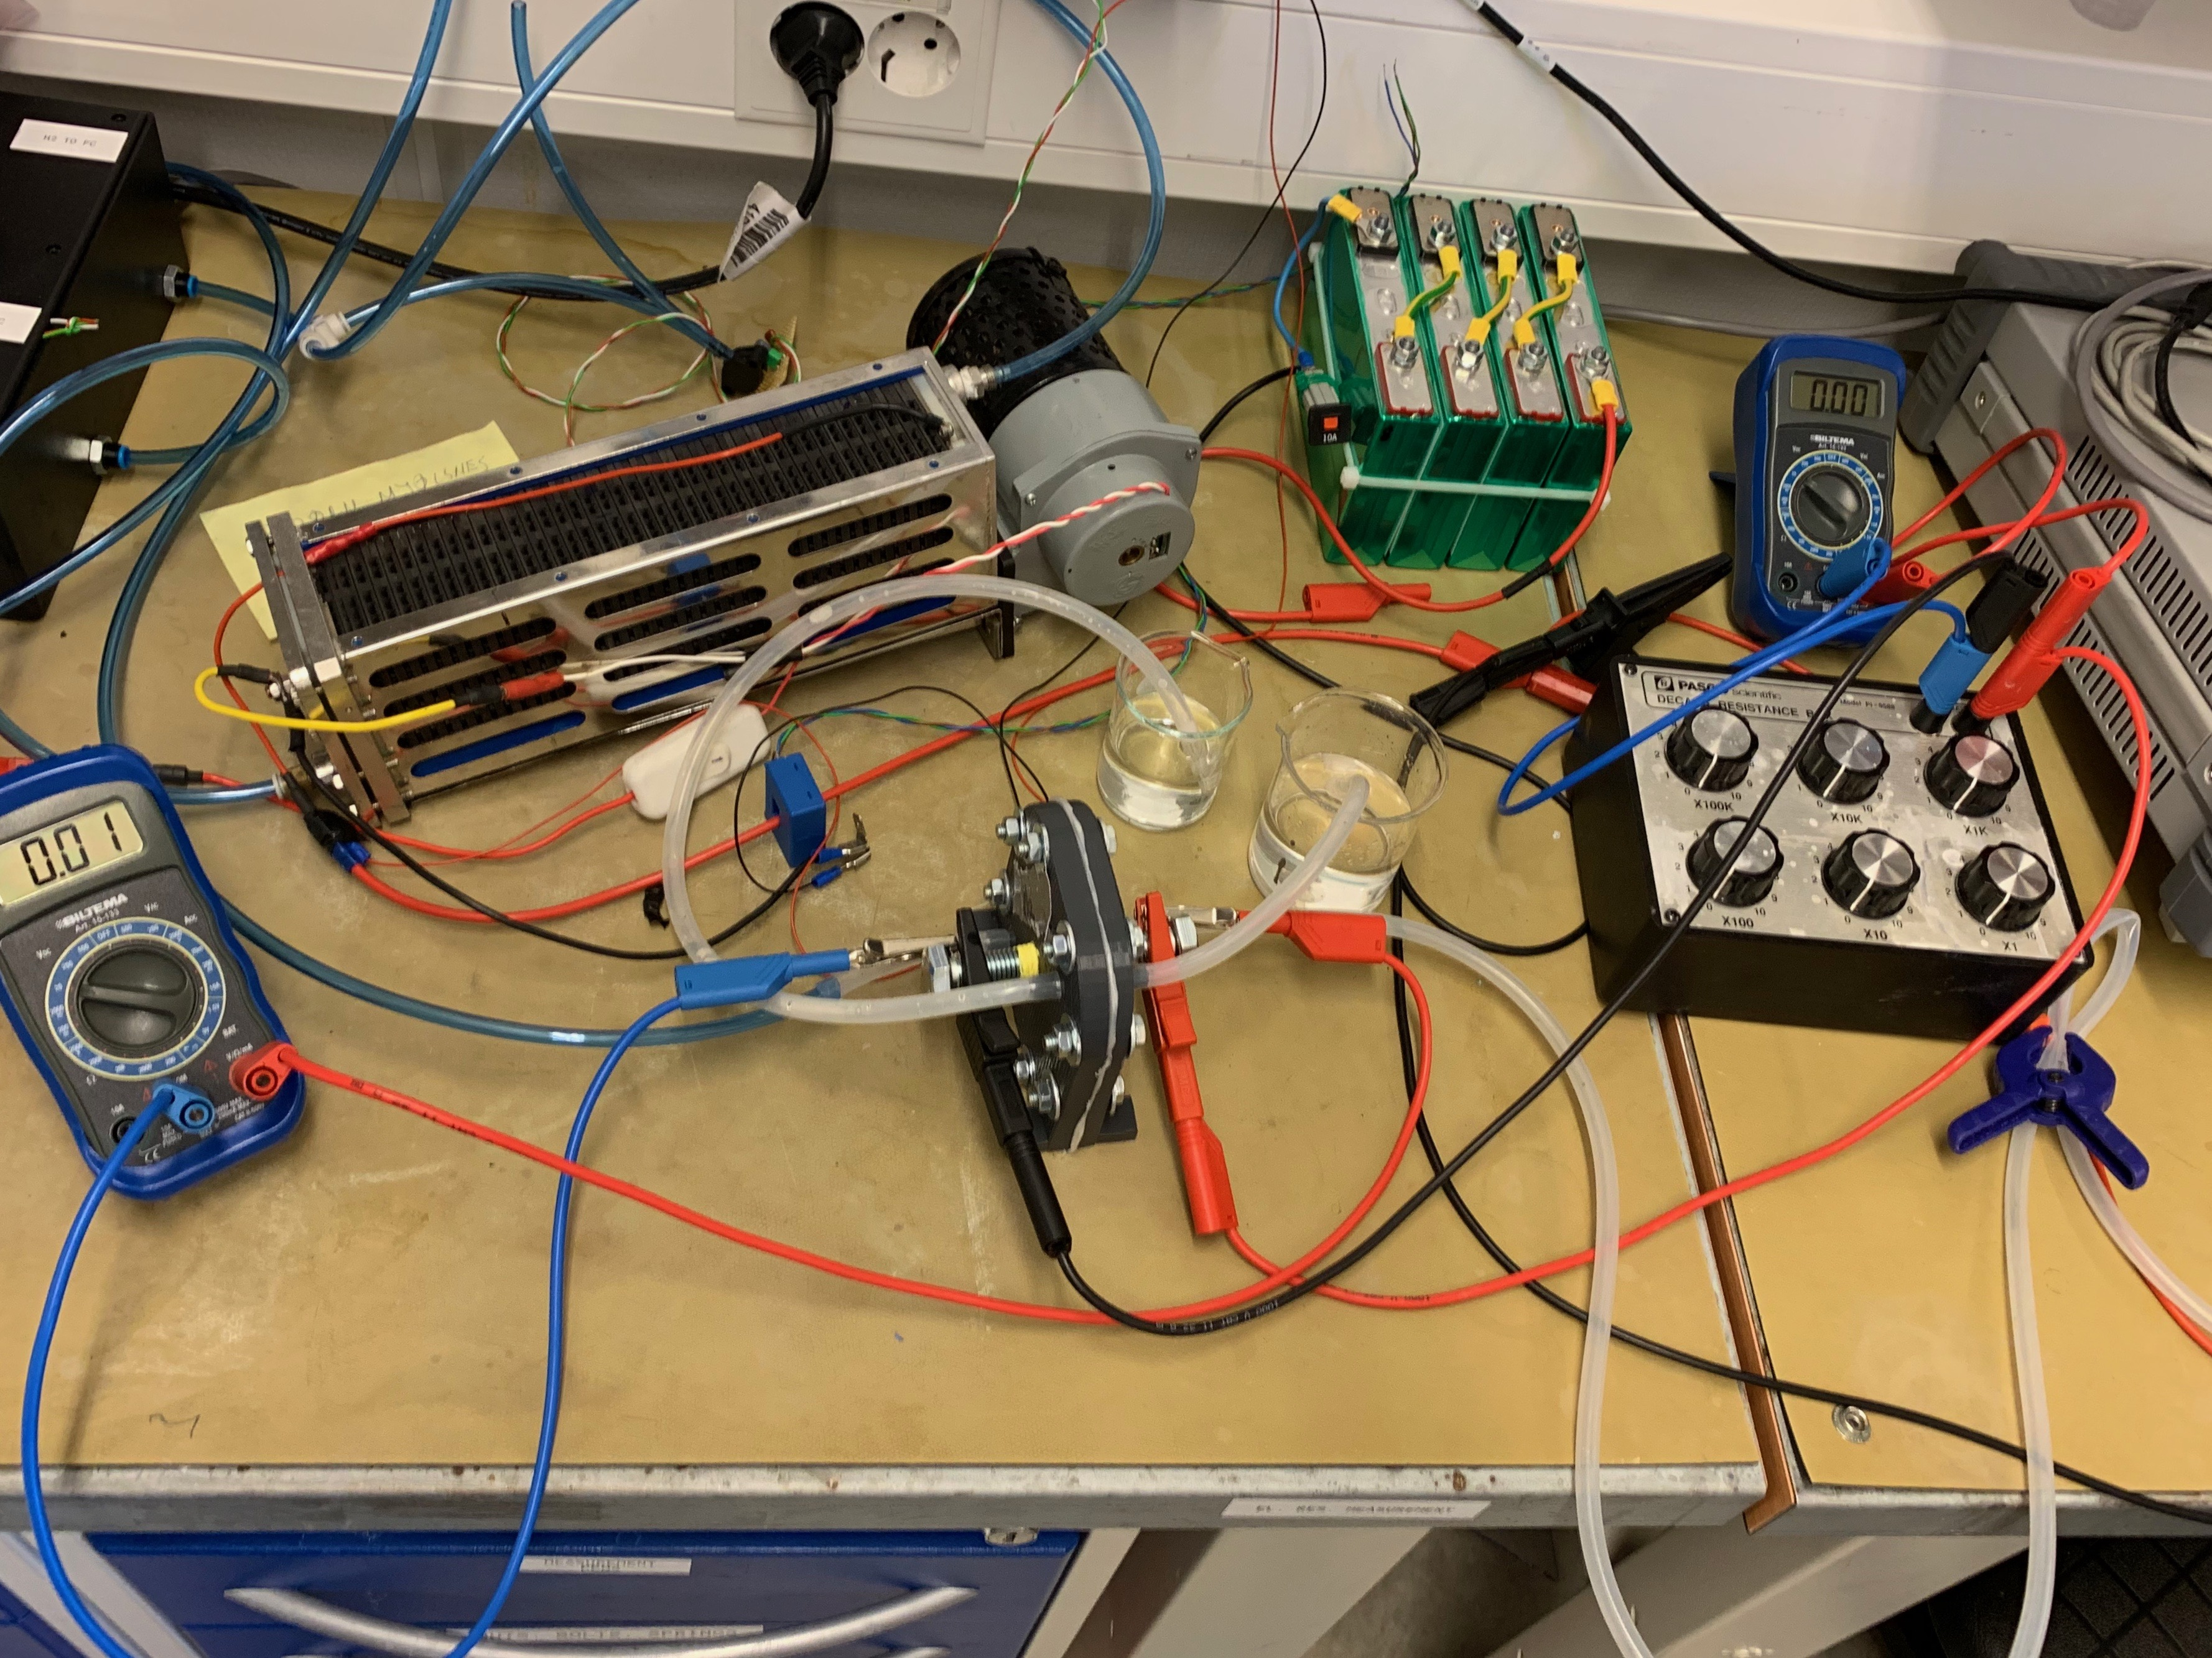
\includegraphics[width=\textwidth]{DIV./Bilder/lab.jpg}
    \caption{Test setup}
    \label{fig:TestSetup}
\end{figure}
